%---------------------------------------------------------------------------%
%-                                                                         -%
%-                           LaTeX Template                                -%
%-                                                                         -%
%---------------------------------------------------------------------------%
%- Copyright (C) Huangrui Mo <huangrui.mo@gmail.com> 
%- This is free software: you can redistribute it and/or modify it
%- under the terms of the GNU General Public License as published by
%- the Free Software Foundation, either version 3 of the License, or
%- (at your option) any later version.
%---------------------------------------------------------------------------%
%->> Document class declaration
%---------------------------------------------------------------------------%
\documentclass[oneside]{Style/ucasthesis}%
%- Multiple optional arguments:
%- [<oneside|twoside|print>]% oneside eprint, twoside eprint, or paper print
%- [fontset=<adobe|none|...>]% specify font set instead of automatic detection
%- [scheme=plain]% thesis writing of international students
%- [draftversion]% show draft version information
%- [standard options for ctex book class: draft|paper size|font size|...]%
%---------------------------------------------------------------------------%
%->> Document settings
%---------------------------------------------------------------------------%

\usepackage[<super>,list,table,math]{Style/artratex}
%- usage: \usepackage[option1,option2,...,optionN]{artratex}
%- Multiple optional arguments:
%- [bibtex|biber]% set bibliography processor and package
%- [<numbers|super|authoryear|alpha>]% set citation and reference style
%- <numbers>: textual: Jones [1]; parenthetical: [1]
%- <super>: textual: Jones superscript [1]; parenthetical: superscript [1]
%- <authoryear>: textual: Jones (1995); parenthetical: (Jones, 1995)
%- <alpha>: textual: not available; parenthetical: [Jon95]
%- [geometry]% reconfigure page layout via geometry package
%- [lscape]% provide landscape layout environment
%- [xhf]% disable header and footer via fancyhdr package
%- [color]% provide color support via xcolor package
%- [background]% enable page background
%- [tikz]% provide complex diagrams via tikz package
%- [table]% provide complex tables via ctable package
%- [list]% provide enhanced list environments for algorithm and coding
%- [math]% enable some extra math packages
%- [xlink]% disable link colors
\usepackage{Style/artracom}% user defined commands
%---------------------------------------------------------------------------%
%->> Document inclusion
%---------------------------------------------------------------------------%
%\includeonly{Tex/Chap_1,...,Tex/Chap_N}% selected files compilation
%---------------------------------------------------------------------------%
%->> Document content
%---------------------------------------------------------------------------%
%-
%-> Titlepage information
%-
\usepackage{pdfpages}


\newcommand{\fun}[1]{\mathrm{#1}}
\newcommand{\vct}[1]{\boldsymbol{#1}}
\newcommand{\mat}[1]{\mathbf{#1}}
\newcommand{\ii}{\hspace{0.1em}\fun{i}\hspace{0.1em}}
\newcommand{\e}{\fun{e}}
\newcommand{\dd}{\fun{d}}
\newcommand{\ve}{\varepsilon}
\newcommand{\lag}{\langle}
\newcommand{\rag}{\rangle}
\newcommand{\llag}{\left\langle}
\newcommand{\rrag}{\right\rangle}
\newcommand{\ts}{\thinspace}
\newcommand{\ls}{\left(}
\newcommand{\rs}{\right)}
\newcommand{\lmi}{\left[}
\newcommand{\rmi}{\right]}
\newcommand{\lb}{\left\{}
\newcommand{\rb}{\right\}}
\newcommand{\ua}{\uparrow}
\newcommand{\da}{\downarrow}
\newcommand{\dg}{\dagger}
\newcommand{\pt}{\partial}
\newcommand{\hoeff}{H_{o}^{\fun{eff}}}

% %---------------------------------------------------------------------------%
%->> Titlepage information
%---------------------------------------------------------------------------%
%-
%-> 中文封面信息
%-
\confidential{}% 密级:涉密论文或延迟公开论文填写
\schoollogo[scale=0.095]{ucas_logo}% 校徽
\title{文献综述-强关联材料的第一性原理计算}% 论文中文题目
\author{论文作者}% 论文作者
\advisor{李四~教授~中国科学院xxx研究所\\}% 指导教师:姓名 专业技术职务 工作单位
%\advisor{指导教师一\\指导教师二\\指导教师三}% 多行指导教师示例
\degree{博士}% 学位:学士、硕士、博士
\degreetype{工学}% 学位类别:理学、工学、工程、医学等
\major{计算机应用技术}% 一级/二级学科专业名称,领域名称需要与学籍信息一致
\institute{中国科学院xxx研究所}% 院系名称
%\institute{中国科学院力学研究所\\流固耦合实验室}% 多行院系名称示例
\date{2023~年~6~月}% 毕业日期:夏季为6月、冬季为12月
%-
%-> 英文封面信息
%-
\TITLE{LaTeX Thesis Template of UCAS}% 论文英文题目
\AUTHOR{Author Name}% 论文作者
\ADVISOR{Supervisor: Professor LI Si}% 指导教师
\DEGREE{Doctor}% 学位:Bachelor, Master, Doctor, Postdoctor。封面据英文学位名称自动切换,需确保拼写准确
\DEGREETYPE{Philosophy}% 学位类别:Philosophy, Natural Science, Engineering, Economics, Agriculture 等
\MAJOR{Computer Application Technology}% 二级学科专业名称
\INSTITUTE{Institute of xxx, Chinese Academy of Sciences}% 院系名称
\DATE{June, 2023}% 毕业日期:夏季为June、冬季为December
%---------------------------------------------------------------------------%
%
\begin{document}
%-
%-> Frontmatter: title page, abstract, content list, symbol list, preface
%-

\frontmatter% initialize the environment
% %---------------------------------------------------------------------------%
%->> Frontmatter
%---------------------------------------------------------------------------%
%-
%-> 生成封面
%-

% \maketitle% 生成中文封面
% \MAKETITLE% 生成英文封面
%-
%-> 作者声明
%-
% \makedeclaration% 生成声明页

\includepdf{Img/Frontpage.pdf}
%-
%-> 中文摘要
%-
\intobmk\chapter*{摘\quad 要}% 显示在书签但不显示在目录
\setcounter{page}{1}% 开始页码
\pagenumbering{Roman}% 页码符号

在强关联材料计算中,电子关联会导致实际数值计算中遇到所谓的“指数墙”困难。为克服这一问题,人们不断发展了各种近似计算方案,从量子力学发展之初建立起的波恩-奥本海默近似,哈特利-福克近似,到后来成为主流计算方案的密度泛函理论,第一性原理计算的性能得到了不断提升。密度泛函理论的主要思路是体系全部物理性质都能够由基态密度唯一确定下来。这一方案的主要问题是囿于平均场图像,难以引入电子关联。为处理这一问题,人们进一步采用引入静态相互作用的 LDA+$U$ 方法来处理关联效应导致的电子局域化等性质,以及引入动态修正的 DFT+DMFT 方案,从而能够在实际计算中得到近藤物理相关性质。

\keywords{第一性原理计算,密度泛函理论,动力学平均场理论}% 中文关键词
%-
%-> 英文摘要
%-
\intobmk\chapter*{Abstract}% 显示在书签但不显示在目录

In strongly correlated material calculations, electronic correlations can lead to difficulties in obtaining accurate numerical results, commonly known as the "exponential wall" problem. To overcome this issue, various approximate computational schemes have been developed over time. These include the Born-Oppenheimer approximation and the Hartree-Fock approximation, which were established in the early stages of quantum mechanics, as well as the density functional theory (DFT), which has become the mainstream computational approach. The performance of first-principles calculations has been continuously improved. The main idea behind the density functional theory is that all physical properties of a system can be uniquely determined by its ground-state density. However, this approach is limited by the mean-field approximation and struggles to incorporate electronic correlations. To address this problem, researchers have introduced methods such as the LDA+U approach, which introduces static interaction to capture localized electronic properties affected by correlation effects, and the DFT+DMFT scheme, which incorporates dynamic corrections. These methods allow for the calculation of Kondo physics-related properties in practical computations.
    %- the current style, comment all the lines in plain style definition.

\KEYWORDS{First Principle Calculation, Density Functional Theory, Dynamical Mean Field Theory}% 英文关键词

\pagestyle{enfrontmatterstyle}%
\cleardoublepage\pagestyle{frontmatterstyle}%

%---------------------------------------------------------------------------%
% title page, abstract
% \fancypagestyle{figureheader}{
%   \fancyhf{}
%   \fancyhead[C]{\footnotesize 图表目录}%此处填写中文标题
%   \fancyfoot[C]{\footnotesize \thepage}% page number
%     \renewcommand{\headrulewidth}{0.8pt}% header rule
%     \renewcommand{\footrulewidth}{0pt}% footer rule
% }
{% content list region
\linespread{1.2}% local line space
\intobmk*{\cleardoublepage}{\contentsname}% add link to bookmark
\tableofcontents% content catalog

% \intobmk*{\cleardoublepage}{图表目录}
\thispagestyle{noheaderstyle}
{
\renewcommand*{\addvspace}[1]{}
\let\oldnumberline\numberline%
\renewcommand{\numberline}{\figurename~\oldnumberline}%
\listoffigures%
}
{
\let\cleardoublepage\relax
\let\clearpage\relax
\renewcommand*{\addvspace}[1]{}
\let\oldnumberline\numberline%
\renewcommand{\numberline}{\tablename~\oldnumberline}%
\listoftables%
}

% \thispagestyle{figureheader}
}
% \intobmk\chapter*{符号列表}% 显示在书签但不显示在目录

\section*{字符}
\nomenclatureitem[\textbf{Unit}]{\textbf{Symbol}}{\textbf{Description}}
\nomenclatureitem[$\Unit{m^{2} \cdot s^{-2} \cdot K^{-1}}$]{$R$}{the gas constant}
\nomenclatureitem[$\Unit{m^{2} \cdot s^{-2} \cdot K^{-1}}$]{$C_v$}{specific heat capacity at constant volume}
\nomenclatureitem[$\Unit{m^{2} \cdot s^{-2} \cdot K^{-1}}$]{$C_p$}{specific heat capacity at constant pressure}
\nomenclatureitem[$\Unit{m^{2} \cdot s^{-2}}$]{$E$}{specific total energy}
\nomenclatureitem[$\Unit{m^{2} \cdot s^{-2}}$]{$e$}{specific internal energy}
\nomenclatureitem[$\Unit{m^{2} \cdot s^{-2}}$]{$h_T$}{specific total enthalpy}
\nomenclatureitem[$\Unit{m^{2} \cdot s^{-2}}$]{$h$}{specific enthalpy}
\nomenclatureitem[$\Unit{kg \cdot m \cdot s^{-3} \cdot K^{-1}}$]{$k$}{thermal conductivity}
\nomenclatureitem[$\Unit{kg \cdot m^{-1} \cdot s^{-2}}$]{$S_{ij}$}{deviatoric stress tensor}
\nomenclatureitem[$\Unit{kg \cdot m^{-1} \cdot s^{-2}}$]{$\tau_{ij}$}{viscous stress tensor}
\nomenclatureitem[$\Unit{1}$]{$\delta_{ij}$}{Kronecker tensor}
\nomenclatureitem[$\Unit{1}$]{$I_{ij}$}{identity tensor}

\section*{算子}
\nomenclatureitem{\textbf{Symbol}}{\textbf{Description}}
\nomenclatureitem{$\Delta$}{difference}
\nomenclatureitem{$\nabla$}{gradient operator}
\nomenclatureitem{$\delta^{\pm}$}{upwind-biased interpolation scheme}

\section*{缩写}
\nomenclatureitem{CFD}{Computational Fluid Dynamics}
\nomenclatureitem{CFL}{Courant-Friedrichs-Lewy}
\nomenclatureitem{EOS}{Equation of State}
\nomenclatureitem{JWL}{Jones-Wilkins-Lee}
\nomenclatureitem{WENO}{Weighted Essentially Non-oscillatory}
\nomenclatureitem{ZND}{Zel'dovich-von Neumann-Doering}

% symbol list, preface content
%-
%-> Mainmatter
%-
\mainmatter% initialize the environment
\renewcommand{\labelenumi}{(\arabic{enumi}) }
\renewcommand{\labelenumii}{(\arabic{enumi}).\arabic{enumii}}
\renewcommand{\labelenumiii}{(\arabic{enumi}).\arabic{enumii}.\arabic{enumiii}}
\renewcommand{\labelenumiv}{(\arabic{enumi}).\arabic{enumii}.\arabic{enumiii}.\arabic{enumiv}}
%---------------------------------------------------------------------------%
%->> Main content
%---------------------------------------------------------------------------%
\renewcommand{\thefigure}{\thechapter-\arabic{figure}}
\renewcommand{\thetable}{\thechapter-\arabic{table}}
\renewcommand{\theequation}{\thechapter-\arabic{equation}}
% \chapter{研究背景}
\section{量子多体系统的“指数墙”问题}
在 1998 年的 Nobel Lecture 上,因发展了密度泛函理论而获得当年诺贝尔化学奖的 H. Kohn 指出, 在实际求解多电子体系的问题时,人们在信息存储和数值计算层面都会遇到所谓的 "指数墙" 问题\cite{Kohn1999}。

在数据存储层面,以金刚石结构为例。元胞中包含两个不等价碳原子,每个原子有四个价电子,如果将空间划分为 $\Delta x\sim 0.1$ 的网格用于存储电子信息,那么仅仅计算一个金刚石元胞,计算机就需要存储 $(10000)^8\sim 10^{32}~\text{bytes}$ 的数据。对于原子数量高达 $10^{23}$ 量级的实际固体材料而言,现有计算机无法处理如此海量的电子信息。

在数值计算层面也存在类似问题,下面举例简要说明。多电子体系的精确哈密顿量为
\begin{equation}
    \hat{H}=\hat{T}_{\text{n}}+\hat{T}_{\text{e}}+\hat{U}_{\text{n-n}}+\hat{U}_{\text{e-e}}+\hat{U}_{\text{n-e}},
\end{equation}
其中五项分别为
\begin{equation}
    \left\{
        \begin{aligned}
            &\hat{T}_{\text{n}}=\sum_{\alpha}-\frac{1}{2M_{\alpha}}\nabla_\alpha^2,\quad &\text{原子核动能项,}\\
            &\hat{T}_{\text{e}}=\sum_i -\frac{1}{2}\nabla_i^2,&\text{电子动能项,}\\
            &\hat{U}_{\text{n}-\text{n}}=\sum_{\alpha<\beta}\frac{Z_{\alpha}Z_{\beta}}{\left| R_{\alpha}-R_{\beta} \right|},&\text{核-核相互作用项},\\
            &\hat{U}_{\text{e-e}}=\sum_{i<j}\frac{1}{\left| r_i-r_j \right|},&\text{电子-电子相互作用项},\\
            &\hat{U}_{\text{n-e}}=\sum_{\alpha i}\frac{-Z_\alpha}{\left| R_\alpha-r_i \right|},&\text{核-电子相互作用项}.
        \end{aligned}\right.
\end{equation}
以水分子为例, 如果保留哈密顿量中的所有项,单个水分子含有三个原子核和十个电子,相互作用项将存在 $C_{13}^2=\frac{13\times 12}{2\times 1}=78$ 项,两个相互作用的水分子就有 $C_{26}^2=\frac{26\times 25}{2\times 1}=325$ 项。当考虑到实际 $10^{23}$ 量级的宏观系统时,相互作用项将指数级增加,多电子体系再一次成为一个难以处理的问题。

为了跨越“指数墙”问题,人们自量子力学框架建立以来,结合实际问题不断提出各种近似方法,探索处理多电子问题的可能途径。下面简要介绍一些重要的近似方法,这些近似虽然有各自的优缺点和局限性,但正是人们持续的尝试与探索,构建起了第一性原理计算的基础。
\section{波恩-奥本海默近似}
波恩-奥本海默近似(Born-Oppenheimer Approximation)的理论基础是原子核的质量 $M$ 比电子质量大三个数量级以上,因此电子与核之间的耦合可以分开\cite{born1927quantum}。当原子核位移时,电子会迅速调整到新的状态,亦即核的运动与电子的运动是相对独立的。因此可以将电子运动受原子核运动的影响作为微扰处理。这种近似方法考虑了当原子核位移时,电子会迅速调整到新的状态,即电子的初态是 $|\psi(0)\rangle=|m(0)\rangle$ 是本征态,则 $t>0$ 时刻电子将保持在相应的瞬时本征态 $|m(t)\rangle$ 上,与量子绝热定理一致,因此也称为\textbf{绝热近似}\cite{Born1928BeweisDA}。

然而,在波恩-奥本海默近似下,多电子系统的总电子数仍然是一个大到难以处理的量,这使得精确求解一个量子多体问题仍然十分困难。因此,人们仍需要进一步寻找近似方法。

\section{哈特利方法}
1927 年哈特利(Hartree)提出一种称为自洽场(self-consistent field)的方法,用于近似计算原子和离子的近似波函数与能量\cite{hartree_1928}。在这一方法中, Hartree 尝试脱离经验参数,直接从最基本的物理原理出发求解不含时多体薛定谔方程,这就是人们常说的从头计算(\textit{ab initio} calculation)方法。但在当时,人们并没有理解这一方法理念,质疑 Hartree 的方法与多体薛定谔方程之间的关系不明确,包含了一些经验主义方法。后来 J. Slater 和 J. Gaunt 各自独立证明了,利用变分原理,Hartree 方法能够应用在作为单粒子波函数直积的试探波函数上\cite{PhysRev.32.339, gaunt_1928}。这为 Hartree 方法提供了更完善的理论框架。

Hartree 所做的近似方法如下。考虑某个电子运动时,它与其他电子的相互作用的运动可以近似看成是它在其他电子的平均密度所产生的电磁场中的运动,这样就得到了一个平均场近似。

假定对第 $i$ 个电子而言,它感受到的其他电子的平均场为 $\hat{g}_i(r)$ ,则库伦相互作用势可以简化为:
\begin{equation}
\hat{U}_{ee}\approx\sum_{i=1}\hat{g}_i(r),
\end{equation}
那么电子的哈密顿量可以写作:
\begin{equation}
\hat{H}\approx\sum_{i=1}\left(-\frac{1}{2}\nabla_i^2+\hat{v}_i+\hat{g}_i\right)\equiv\sum_{i=1}\hat{H}_i.
\end{equation}
这样,整个哈密顿量在平均场近似下就可以分离变量,多电子的薛定谔方程可以化简为 $N$ 个单电子薛定谔方程:
\begin{equation}
\hat{H}_i\phi_n(r_i)=\epsilon_n\phi_n(r_i),\quad \Psi(\{r_i\})=\prod_i \phi_i(r_i).
\end{equation}
相应的能量平均值是:
\begin{equation}
\begin{aligned}
\langle\hat{H} \rangle_{\mathrm{Hatree}}=&\langle\Psi(\{r_i\})|\left(\sum_{i=1}\hat{h}_i+\hat{U}_{e-e} \right)\\
=&\sum_{i=1}\langle\phi_i(r)|\hat{h}_i|\phi_i(r)\rangle+\frac{1}{2}\sum_{i\ne j}\langle\phi_i(r)\phi_j(r')\Big|\frac{1}{|r-r'|}\Big|\phi_i(r)\phi_j(r')\rangle.
\end{aligned}
\end{equation}
构造一个总能量附加波函数归一化条件的泛函,泛函对$\langle \phi_i(r)|$取变分极小:
\begin{equation}
\delta\left[ \langle\hat{H}\rangle_{\mathrm{Hatree}} -\sum_i E_i \left( \langle\phi_i|\phi_i\rangle-1\right)\right]=0,
\end{equation}
带入 $\langle\hat{H}\rangle_{\mathrm{Hatree}}$ 具体表达式,得到:
\begin{equation}
\sum_{i=1}\langle\delta \phi_i(r)|\hat{h}_i|\phi_i(r) \rangle+\sum_{i\ne j}\langle\delta \phi_i(r)\phi_j(r')\Big|\frac{1}{|r-r'|} \Big|\phi_i(r)\phi_j(r') \rangle-\sum_iE_i\left(\langle\delta\phi_i(r)|\phi_i(r) \rangle \right)=0,
\end{equation}
上式相当于是遍历 $i$ 的 $N$ 个独立方程(取消对 $i$ 的求和):
\begin{equation}
\langle\delta \phi_i(r)|\hat{h}_i|\phi_i(r) \rangle+\sum_{j(\ne i)}\langle\delta \phi_i(r)\phi_j(r')\Big|\frac{1}{|r-r'|} \Big|\phi_i(r)\phi_j(r') \rangle-E_i\left(\langle\delta\phi_i(r)|\phi_i(r) \rangle \right)=0,
\end{equation}
整理得到:
\begin{equation}
\left\langle\delta\phi_i(r)\left|\left\{\hat{h}_i+\sum_{j(\ne i)}\langle\phi_j(r')|\frac{1}{|r-r'|}|\phi_j(r') \rangle-E_i \right\} \right|\phi_i(r) \right\rangle=0,
\end{equation}
由于 $\delta\phi_i(r)$ 任意,所以方程右半部分恒为零,得到有效势的单电子方程:
\begin{equation}
\left.\left.\left\{\hat{h}_i+\sum_{j(\ne i)}\langle\phi_j(r')|\frac{1}{|r-r'|}|\phi_j(r') \rangle-E_i \right\} \right|\phi_i(r) \right\rangle=0,
\end{equation}
整理得到 Hartree 方程:
\begin{equation}
\left(-\frac{1}{2}\nabla_i^2+\hat{v}_i+\hat{g}_i \right)|\phi_i(r)\rangle=E_i|\phi_i(r)\rangle,
\end{equation}
其中 $\hat{g}_i$ 常称为 Coulomb 项或 Hartree 项:
\begin{equation}
\hat{g}_i(r)=\sum_{j(\ne i)}\int\mathrm d r'\frac{|\phi_j(r')|^2}{|r-r'|}.
\end{equation}
需要对方程作自洽计算,迭代计算上两式中的 $|\phi_i(r)\rangle$ 和 $\hat{g}_i$ 。这样就将多电子问题化为了单电子问题。

然而,1930 年,Slater 和 Fock 分别独立指出, Hartree 方法不能满足费米子波函数的反对称性,从而无法考虑 Pauli 不相容原理\cite{PhysRev.35.210.2, Fock1930}。
\section{哈特利-福克方法}
在 1935 年,Hartree 在之前的方法和 Fock 的方法的基础上,重新构造了更合适的算法来处理量子多体计算问题,利用满足交换反称的 Slater 总波函数替代了 Hartree 近似的波函数,这被称为哈特利-福克(Hartree-Fock)方法\cite{Hartree1935}。这样, Pauli 不相容原理就被自然地引入到了波函数基底中:
\begin{equation}
\Psi(r_1,r_2,\cdots,r_N)=\frac{1}{\sqrt{N!}}
\left|
\begin{array}{ccccc} 
    \phi_1(r_1)  &  \phi_2(r_1)   & \cdots & \phi_N(r_1) \\ 
   \phi_1(r_2)  &  \phi_2(r_2)   & \cdots & \phi_N(r_2)\\ 
    \vdots  &  \vdots   &\vdots &\vdots\\
    \phi_1(r_N) &\phi_2(r_N)&\cdots&\phi_N(r_N)
\end{array}
\right| .
\end{equation}
变分方法同上 Hatree 方法,得到 Hatree-Fock 本征方程:
\begin{equation}
\hat{f}(r_1)\phi_i(r_1)=\epsilon_i\phi_i(r_1),
\end{equation}
其中 $\hat{f}(r_1)$ 是 Fock 算符:
\begin{equation}
\hat{f}(r_1)=\hat{h}(r_1)+\sum_{a}\left[\hat{J}_a(r_1)-\hat{K}_a(r_1) \right],
\end{equation}
其中单粒子算符项 $\hat{h}(r_1)$ 定义与上一问相同,库仑算符 $\hat{J}_a(r_1)$ 定义为:
\begin{equation}
\begin{aligned}
\hat{J}_a(r_1)\phi_b(r_1)=&\phi_b(r_1)\int|\phi_a(r_2)|^2\frac{1}{|r_1-r_2|}\mathrm d r_2\\
=&\phi_b(r_1)\int\rho_a(r_2)\frac{1}{|r_1-r_2|}\mathrm d r_2,
\end{aligned}
\end{equation}
交换算符 $\hat{K}_a(r_1)$ 定义为:
\begin{equation}
\hat{K}_a(r_1)\phi_b(r_1)=\phi_a(r_1)\int\phi_a^*(r_2)\phi_b(r_2)\frac{1}{|r_1-r_2|}\mathrm{d} r_2.
\end{equation}
对非相互作用体系,$N$ 个电子的每一个满足同样的薛定谔方程,处于平等地位,解单粒子方程可以得到足够多的单粒子态,所有 $N$ 个电子按照能级逐次填充这些单粒子。

在 Hartree-Fock 近似下,体系的总能可以表示为
\begin{equation}
E_{\mathrm{HF}}=\sum_i^N H_i+\frac{1}{2}\sum_{i,j}^N(J_{ij}-K_{ij}),
\end{equation}
电子轨道能量是:
\begin{equation}
\langle\phi_a|\hat f_a|\phi_a\rangle=\epsilon_a.
\end{equation}
总能量可以表示成:
\begin{equation}
\begin{aligned}
E_{\mathrm{HF}}=&\sum_{i=1}^NH_i+\frac{1}{2}\sum_{ij}^N(J_{ij}-K_{ij})\\
=&\sum_i\epsilon_i-\sum_{ij}(J_{ij}-K_{ij})+\frac{1}{2}\sum_{ij}^N(J_{ij}-K_{ij})\\
=&\sum_i\epsilon_i-\frac{1}{2}\sum_{ij}(J_{ij}-K_{ij}),
\end{aligned}
\end{equation}
可见,HF 总能量不是单粒子轨道能量之和。Koopmans 定理表明,在这一近似下,电子轨道能量应等于电子离化能。

Hartree-Fock 近似使得多电子问题变得能够求解。但直到 1950 年电子计算机被发明出来之前,这一方法所需要的计算资源都远超出当时的计算水平。因此当时 Hartree-Fock 方法只能应用于带有球对称性的原子系统\cite{PhysRev.81.385}。

由于 Hartree 方法和 Hartree-Fock 方法都采用了平均场近似,忽略了电子关联,因此在相互作用电子系统中,计算结果将存在较大偏差。针对这一问题的修正统称为 Post Hartree-Fock 方法,包括 Møller–Plesset (MP)微扰理论\cite{PhysRev.46.618}、组态相互作用(Configuration Interaction, CI)修正\cite{DAVIDSHERRILL1999143}等方法。

在 Hartree-Fock 方法发展起来的同时,人们还发展出了密度泛函理论(Density Functional Theory, DFT),这是 Hartree-Fock 方法的另一种替代方案,它将电子密度作为处理多体问题的最基本变量。在 DFT 计算框架下人们能够同时处理交换能和关联能。在强关联电子计算中,人们通常倾向于从 DFT 计算出发,在此基础上利用 DFT+U、DFT+DMFT 等方法进一步考虑电子关联。下一小节将具体介绍密度泛函理论的发展和基本框架。
% \chapter{密度泛函理论}
密度泛函理论(Density Functional Theory, DFT)是目前在材料计算中使用最广泛的一种第一性原理计算方法。与传统的 Hartree-Fock 理论(只考虑了交换能)以及各种考虑进电子关联的 Post-Hartree-Fock 衍生方法相比,DFT 的计算成本相对更低。最早尝试利用密度泛函进行第一性原理计算的是 1927 年 L. Thomas 和 E. Fermi 等人提出的 Thomas-Fermi 模型,这一方法尝试仅使用电子密度来计算量子体系,独立于波函数理论\cite{Fermi1927, Thomas_1927}。为了引入泡利不相容原理,1930 年 P. Dirac 在 Thomas-Fermi 理论中又引入了一项交换能\cite{dirac_1930}。但这一方法给出的电子动能项密度泛函形式过于简单,不能很好地准确描述电子动能项,因此在 Thomas-Fermi-Dirac 理论提出之后,并没有得到广泛应用。后来在此基础上发展起来的密度泛函理论(Density Functional Theory, DFT)使用电子波函数计算动能项,这样就避免了动能项没有精确泛函的问题。同时,密度泛函理论把动能项和电子间库仑相互作用的误差项都放在了能量占比较小的交换关联势中,降低了系统误差。下面逐一介绍作为密度泛函理论出发点的 Thomas-Fermi-Dirac 理论以及密度泛函理论方案的基本原理。
\section{Thomas-Fermi-Dirac 近似及其推广}
Thomas-Fermi 近似认为系统中的电子动能项可以通过将空间划分为小格子,每一个小格子的动能认为是依赖于密度泛函的全同电子气动能,即有
\begin{equation}
    T_{\text{T-F}}=C_{\text{F}}\int\text{d}r^3 \rho^{5/3},\quad C_{\text{F}}\approx 2.871.
\end{equation}
在这一近似下,能量泛函就可以相应地表示为 
\begin{equation}
    E_{\text{T-F}}=C_{\text{F}}\int\text{d}r^3 \rho^{5/3}+\int v(\boldsymbol{r})\rho(\boldsymbol{r})\text{d}r^3+\frac{1}{2}\iint\frac{\rho(\boldsymbol{r}_1)\rho(\boldsymbol{r}_2)}{\left| \boldsymbol{r}_1-\boldsymbol{r}_2 \right|}\text{d}\boldsymbol{r}_1\boldsymbol{r}_2.
\end{equation}
为考虑进电子的交换反对称性质,狄拉克进一步引入交换积分 
\begin{equation}
    K_{ij}=-\int\frac{\phi^*_{k_1}(\vct{r}_1)\phi^*_{k_2}(\vct{r}_2)\phi_{k_1}(\vct{r}_2)\phi_{k_2}(\vct{r}_1)}{\left| \vct{r}_1-\vct{r}_2 \right|}\dd\vct{r}_1\dd\vct{r}_2,
\end{equation}
这样,就得到了 Thomas-Fermi-Dirac 能量泛函的表达式 
\begin{equation}
    \begin{aligned}
        E_{\text{T-F}}=&C_{\text{F}}\int\text{d}r^3 \rho^{5/3}+\int v(\boldsymbol{r})\rho(\boldsymbol{r})\text{d}r^3\\
        &+\frac{1}{2}\iint\frac{\rho(\boldsymbol{r}_1)\rho(\boldsymbol{r}_2)}{\left| \boldsymbol{r}_1-\boldsymbol{r}_2 \right|}\text{d}\boldsymbol{r}_1\dd\boldsymbol{r}_2-C_X\int\dd\rho^{4/3}(\vct{r})\dd\vct{r}.
    \end{aligned}
\end{equation}
这一近似方法使得人们能够有效处理相互作用电子系统。

在这一计算方案中,动能项的密度泛函形式未知,这导致在实际计算中会产生较大的动能项误差。由于没有考虑电子关联,交换能也存在误差。E. Teller 在 1962 年指出,Thomas-Fermi 理论计算得到的任何分子能量都会高于组成这一分子的原子总能,因此这一方案不能用来计算分子成键过程\cite{RevModPhys.34.627}。

密度泛函理论起源于 Thomas-Fermi-Dirac 理论,人们利用 Hohenberg-Kohn 定理将体系的总能量是密度的泛函这一概念加以推广,证明了所有可观测量都是密度的泛函\cite{PhysRev.136.B864}。这一理论使用电子波函数来计算动能项,计算精度高,避免了动能项没有精确泛函的问题,同时把动能项和电子间库仑相互作用的误差都放在交换关联势中,这部分能量比较小。因此相比于 Thomas-Fermi-Dirac 理论,DFT 之后得到了更广泛的应用。下面简单介绍 DFT 的基本原理和计算方案。
\section{基本理论}
1964 年,P. Hohenberg 和 W. Kohn 在非均匀电子气理论的基础上,给出了两条定理:
\begin{theorem}
    在相互作用电子系统中,除了常数项之外,外势场 $V_{\fun{ext}}(\vct{r})$ 可以由基态电子密度 $n_0(\vct{r})$ 唯一确定。
\end{theorem}
\begin{theorem}
    基态总能量泛函 $E[n]$ 可以由基态电子密度 $n_0(\vct{r})$ 和任意给定的外势 $V_{\fun{ext}}(\vct{r})$ 唯一地确定下来。
\end{theorem}
利用反证法(对于定理一:假设同一个基态电子密度 $N_0(\vct{r})$ 可以确定两个不同的外势场;对于定理二:假设有两套基态密度 $n_0(\vct{r})$ 可以确定同一个基态总能量泛函)很容易证明这两条定理\cite{martin_2004},此处不加以赘述。根据这两条定理,基态电子密度就能够唯一地确定体系的哈密顿量(除了常数项),这样体系的全部多体波函数也能够确定下来,这样就得到了密度泛函理论框架中重要的一点,那就是体系的全部物理性质都能够由基态密度 $n_0(\vct{r})$ 唯一地确定下来。

由于两条定理都能被严格证明,证明过程不用取任何近似,因此 DFT 的原始理论本身是精确的。但在实际的物理体系中,只有外势场项的密度泛函表达式是精确已知的,动能项和电子-电子相互作用项并没有精确的密度泛函表达式。这导致原始的 DFT 无法被应用到实际计算中。

为处理这一困难,1965 年 W. Kohn 和 L. Sham 在 DFT 基础上利用一套等效的无相互作用参考电子系统(Kohn-Sham auxiliary system)近似描述多电子系统\cite{PhysRev.140.A1133}。这一方案假定无相互作用的参考电子系统与有相互作用的多电子系统具有相同的基态电子密度,通过求解参考电子系统,就可以得到真实的多电子系统的基态能量和基态电荷密度,是一种近似方案。

在 KS 方程中,参考电子系统的动能泛函是可以求解出来的,库仑相互作用可以使用平均场近似,其他误差都放在交换关联中,其中包含交换能、关联能、电子动能的误差以及库伦势的自相互作用修正。下一小节将具体介绍 Kohn-Sham 框架下的 DFT 基本方程和迭代计算流程。
\section{Kohn-Sham DFT}
Kohn-Sham DFT 的两条基本假设如下。
\begin{itemize}
    \item[(1)] 多电子系统的基态电荷密度可以与一组无相互作用电子系统的基态电荷密度对应起来。人们一般称这一表示方法为“无相互作用 $V$ 可表示性(non-interacting-V-representability)”\cite{ENGLISCH1983253}。这一假设并没有严格的理论证明。
    \item[(2)] 无相互作用的参考电子系统哈密顿量由单电子动能项和等效的局域势场项 $V_{\fun{eff}}^{\sigma}(\vct{r})$ 构成。这样,真实系统的电荷密度就能够写成一些无相互作用波函数密度之和。
\end{itemize}

在这两条基本假设下,实际多电子体系的计算就可以等效地在一个无相互作用粒子系统中展开。参考系统中某一位置处的电荷密度可以表示为
\begin{equation}
    n(\vct{r})=\sum_{\sigma}n(\vct{r},\sigma)=\sum_{\sigma}\sum_{i=1}^{N^\sigma}\left| \psi_i^{\sigma}(\vct{r}) \right|,
\end{equation}
对应的无相互作用系统的动能可以表示为 
\begin{equation}
    T_s=-\frac{1}{2}\sum_{\sigma}\sum_{i=1}^{N^{\sigma}}\llag \psi_i^\sigma \right| \nabla^2 \left| \psi_i^\sigma \rrag = \frac{1}{2}\sum_{\sigma}\sum_{i=1}^{N^\sigma}\int\dd^3 r\left| \nabla \psi_i^\sigma (\vct{r}) \right|,
\end{equation}
然后定义库仑能(也常被称为 Hartree 能)
\begin{equation}
    E_{\fun{Hartree}}[n]=\frac{1}{2}\int\dd^3 r\dd^3 r' \frac{n(\vct{r})n(\vct{r}')}{|\vct{r}-\vct{r}'|},
\end{equation} 
总的 Kohn-Sham 能量泛函表达式就可以表示为 
\begin{equation}
    E_{\fun{KS}}=T_s[n]+\int\dd\vct{r}V_{\fun{ext}}(\vct{r})n(\vct{r})+E_{\fun{Hartree}}[n]+E_{\fun{xc}}[n].
\end{equation}
在这一思想下,波函数的反对称性带来的相互作用被归为交换项;原始体系的关联相互作用统一归为关联项,这两项补充在交换关联能 $E_{\fun{xc}}[n]$ 中。这样,形式上 Kohn-Sham 能量泛函表达式就是严格成立的。

在数值计算求解 KS 方程的过程中,人们往往需要对波函数基底作截断。采用合适的基底可以降低基底的阶数,从而减少计算量。在 WIEN2k 程序\cite{WIEN2k}中使用的是线性缀加平面波(Linearized Augmented plane wave, LAPW)基底,这一方案在靠近原子核附近划定一个范围,称为 Muffin-tin 球,球内使用球谐函数展开,球外使用平面波展开,这样就能够较好地同时描述原子核附近剧烈变化的波函数和远离原子核处平缓的波函数\cite{lapw}。LAPW 是目前计算晶体电子结构最精确的方案之一。

如果体系的交换关联泛函已知,那么基态能和多电子系统的电荷密度就能够通过求解 Kohn-Sham 单电子方程得到。对于大部分交换关联泛函形式未知的实际系统,人们给出各种近似方案来表示这一项,这也使得计算多电子系统变得可能。事实上,密度泛函理论的一个重要方向就是不断发展更准确的交换关联形式,使计算结果更可靠。

在 KS 方程中,最早使用的交换关联泛函采用的是局域密度近似(Local Density Approximation, LDA),这一方案的思想仍然基于均匀电子气,认为交换关联泛函的每一点取值只和这一点的电荷密度有关。考虑到交换能和关联能的物理含义不同,需要分开处理,有
\begin{equation}
    E_{\fun{xc}}[n]=E_{\fun{x}}[n]+E_{\fun{c}}[n].
\end{equation}
在 LDA 近似下,交换项和关联项可以分别表示为 
\begin{equation}
    E_{\fun{x}}^{\fun{LDA}}[n]=\int \dd^3 r\ n(\vct{r})\epsilon_{\fun{x}}[n(\vct{r})],\quad E_{\fun{c}}^{\fun{LDA}}[n]=\int \dd^3 r\ n(\vct{r})\epsilon_{\fun{c}}[n(\vct{r})],
\end{equation}
其中 $\epsilon_{\fun{x}}[n(\vct{r})]$ 和 $\epsilon_{\fun{c}}[n(\vct{r})]$ 是密度为 $n$ 的电子气中单个电子对应的交换能和关联能,交换能可以严格推导得到,但关联能没有严格的解析表达式。1980 年, D. Ceperley 和 B. Alder 等人利用量子蒙特卡洛方法得到了较为精确的关联能数值结果\cite{PhysRevLett.45.566},后来人们对这一数值结果进行参数化,得到了两种关联能量密度的具体表达式\cite{PhysRevB.23.5048,PhysRevB.45.13244}。

但是对于电子势场在空间中变化剧烈的体系,LDA 近似就不再适用。在此基础上,人们考虑添加一项密度梯度修正项,这样就得到了各种广义梯度近似(Generalized Gradient Approximation, GGA)的交换关联泛函,比如在实际计算中常使用的 B88\cite{B88},PW91\cite{PW91},PBE\cite{PBE} 泛函等。然而 GGA 近似仍然是一个局域泛函,无法考虑长程关联,所以这种近似方案仍然不能很好地处理强关联电子系统。
\begin{figure}[H]
    \vspace{13pt} % 调整图片与上文的垂直距离
    \centering
    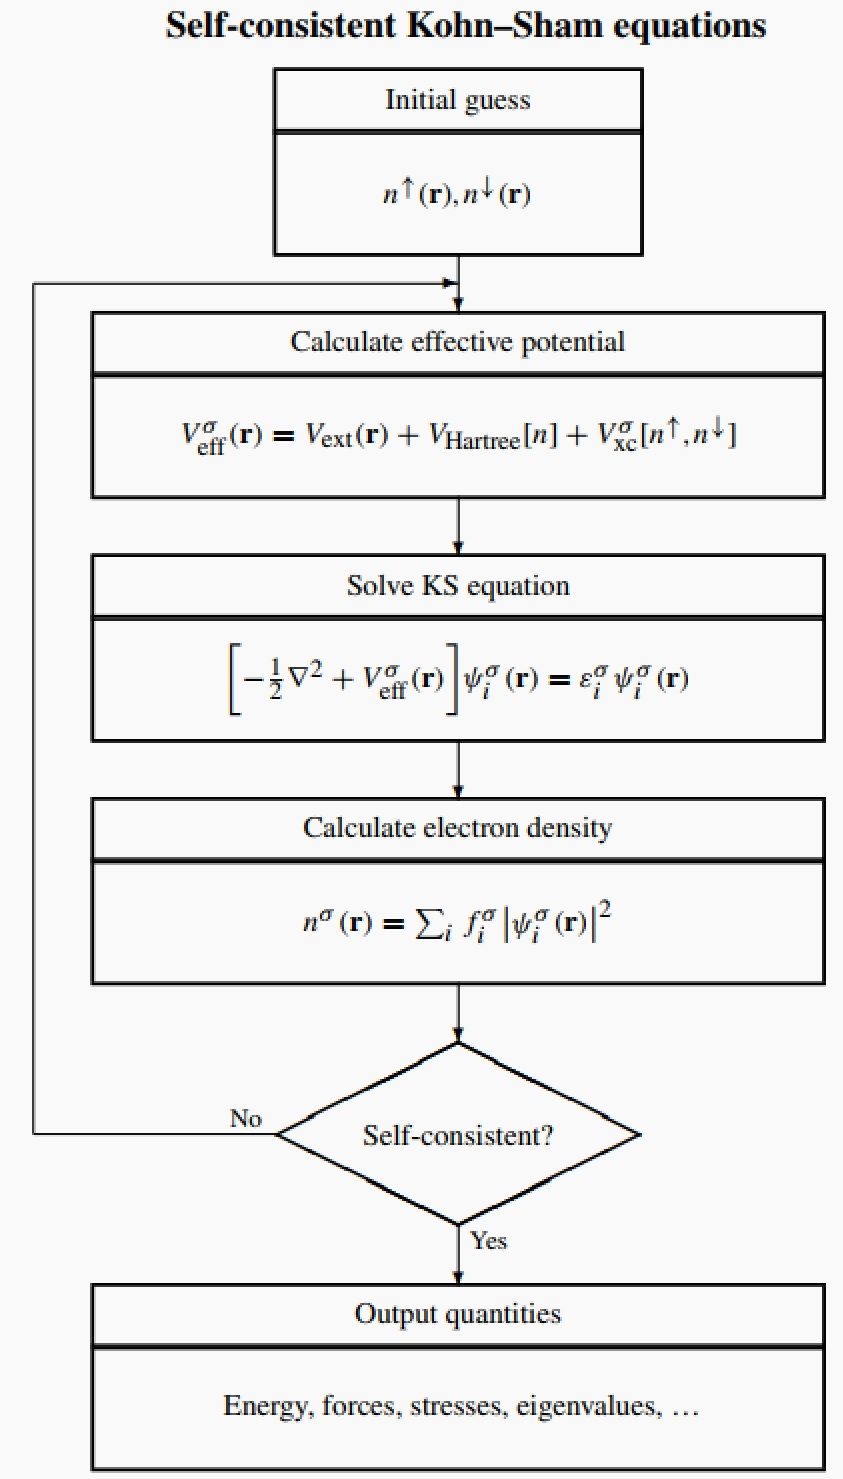
\includegraphics[width=3.5in]{Img/ks-scf.png}
    \caption{KS-DFT 自洽计算流程示意图\cite{martin_2004}。}
    \label{KS-scf} 
\end{figure}
DFT 自洽计算的一般流程如图 \ref{KS-scf} 所示,首先根据初始输入的晶格信息等参数计算出初始电荷密度 $n^{\ua}(\vct{r})$ 和 $n^\da(\vct{r})$,利用这一电荷密度计算出 DFT 的等效外势场 $V_{\fun{eff}}^{\sigma}(\vct{r})$(对应 WIEN2k 的 lapw0 程序),接着利用这一势场求解单电子近似下的 KS 方程(对应 lapw1 程序)得到本征值和本征波矢,再利用这些计算结果得到体系的费米能和新的电荷密度(对应程序 lapw2),如果新旧电荷密度不收敛,则使用 mixer 程序混合新旧电荷密度重复上述步骤,如果电荷收敛,则完成自洽计算,可以进一步使用计算得到的电荷密度分析各种实际物理量。

在强关联电子体系的计算中,密度泛函理论会出现较大问题。例如 3$d$ 电子的过渡金属氧化物、4$f$ 电子的稀土氧化物、5$f$ 电子的锕系元素氧化物中,电子关联带来的效应不能被忽略。一个 DFT 失效的典型问题是对 Mott 绝缘体的预测。DFT 电子结构计算通常会给出金属基态,但实验结果是带隙较宽的绝缘体。这是因为 Mott 绝缘体中通常具有部分填充的 $d$ 电子壳层,其中存在很强的库仑相互作用。如果库仑相互作用 $U$ 大于带宽 $W$,电子将趋于局域化,因此体系会出现由关联效应导致的绝缘性质。密度泛函理论这种单电子近似方法不能很好地描述这种关联性质。一些简单的修正方法能够一定程度上改进这一缺陷。最常用的方法是在电子的 $d$ 或 $f$ 轨道的势能项中引入库仑相互作用项,这被称为 LDA+$U$ 方法。下面简单介绍一下这一方法的基本思路。
\section{LDA+$U$}
在 LDA+$U$ 方法中,相互作用项定义为 
\begin{equation}
    H_U\equiv \sum_{\sigma\sigma'}\sum_{mm''m'm'''}U_{mm''m'm'''}a_{m\sigma}^\dg a_{m''\sigma'}^\dg a_{m'''\sigma'}^{ }a_{m'\sigma}^{ },
\end{equation}
其中 
\begin{equation}
    U_{mm''m'm'''}\equiv \frac{1}{2}\llag mm''\left| V_{ee} \right| m'm''' \rrag.
\end{equation}
如果将体系的电荷密度划分为弱关联和强关联两部分,弱关联部分用 $\rho$ 表示,强关联部分用 $n$ 表示,可以将能量泛函写成下面的形式:
\begin{equation}
    E^{\fun{LDA}+U}[\rho,n]=E^{\fun{LDA}}[\rho]+E^{U}[n]-E_{\fun{dc}}[n],
\end{equation}
其中 $E_{\fun{dc}}$ 称为双计数项,用于扣除前两项的重叠部分。双计数项目前并没有严格的数学形式,针对不同体系人们采用了不同的双计数项方案,例如在弱关联和半导体系统中适用的 AMF 方案\cite{PhysRevB.44.943,PhysRevB.49.14211}、在接近整数占据的体系中适用的 FLL 方案\cite{PhysRevB.48.16929}、AMF 和 FLL 的插值混合方法\cite{PhysRevB.67.153106}、以及能够对自相互作用项更好修正的方案\cite{PhysRevB.76.033102}等。

然而 LDA+$U$ 方法实际上引入的是静态的相互作用,这一般会高估相互作用效应,并且在平均场意义下无法得到强关联体系的近藤物理。为了克服这一局限性,人们需要在平均场理论的基础上进一步考虑动态效应的修正。动力学平均场理论就是这样一种超越平均场理论的方案,通过将密度泛函理论与动力学平均场理论结合,人们可以在实际材料中计算得到近藤物理的相关性质。下面简要介绍动力学平均场理论的主要方法,以及将密度泛函理论与动力学平均场理论结合的计算方案。

% \chapter{动力学平均场理论(DMFT)}
动力学平均场理论(Dynamical Mean Field Theory, DMFT)的核心思想是将晶格模型自洽地映射为单杂质量子模型,将难以求解的晶格问题转化成量子杂质问题,从而有效降低多体问题的自由度。在处理量子杂质模型时,由于杂质哈密顿量并不会因为晶格模型的不同类型而发生较大变化,因此这一方法的优势是可以处理不同的晶格问题,可以进一步与真实的材料体系计算相结合,很大程度上扩展了强关联材料的计算领域。
\section{模型映射}
为了将晶格模型的性质映射到单杂质模型中,一个直接的方式是扣除晶格模型的一个格点,利用路径积分将其他格点积分掉,得到与单杂质模型数学形式相同的有效作用量。文献中一般称这种推导方法为空腔法(cavity method)\cite{RevModPhys.68.13}。下面从经典 Ising 模型出发,简要介绍空腔法的思路,并具体推导由 Hubbard 模型到单杂质 Anderson 模型的映射。
\subsection{Ising model}
首先以经典 Ising 模型为例, 推导空腔的有效哈密顿量。 Ising 模型的哈密顿量为 
\begin{equation}
    \begin{aligned}
        H=&-\sum_{\langle ij \rangle}J_{ij}S_iS_j-h\sum_iS_i\\
        \equiv&-h_oS_o-\sum_i J_{io}S_oS_i+H^{(o)},
    \end{aligned}
\end{equation}
其中 $J_{ij}>0$ 是最近邻铁磁相互作用, $\sum_{\lag ij \rag}$ 是对最近邻格点对求和, 自旋取 $S_i=\pm 1$。式中第二行将哈密顿量分成三项: 第一项是挖去一个格点 $o$ 之后, $o$ 格点的哈密顿量 $H_o$。第二项是 $o$ 与格点的耦合项 $\Delta H$, 格点周围剩余的格点称为空腔, 哈密顿量是式中第三项 $H^{(o)}$。空腔法的模型如图所示。
\begin{figure}[H]
    \vspace{13pt} % 调整图片与上文的垂直距离
    \centering
    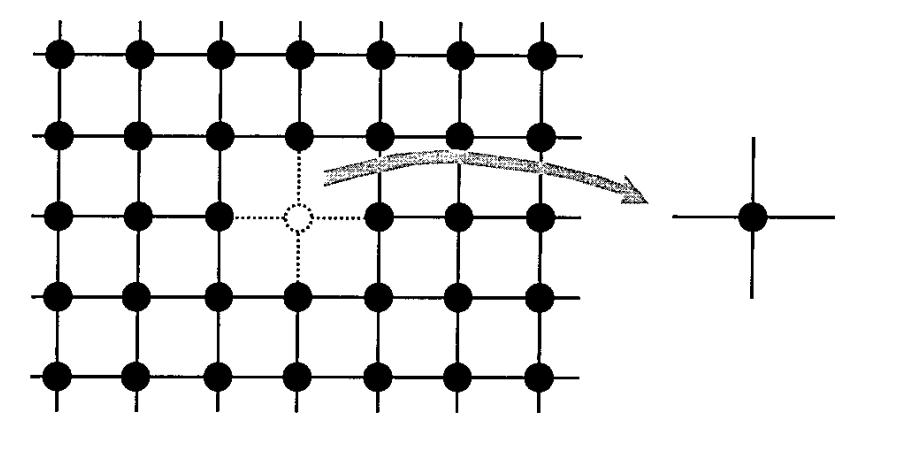
\includegraphics[width=5in]{Img/cavity-method.png}
    \caption{在格点模型中挖去一个格点 $o$ 以及 $o$ 和其他格点的相互作用键} 
\end{figure}
定义作用在格点 $i$ 上的场 $\eta_i$:
\begin{equation}
    \eta_i\equiv J_{io}S_o,
\end{equation}
于是哈密顿量可以改写为 
\begin{equation}
    \left\{
        \begin{aligned}
            H&=H_o+H^{(o)}+\Delta H,\\
            H_o&=-h_oS_o,\\
            \Delta H&=-\sum_{i\ne o}J_{io}S_oS_i\equiv\sum_i\eta_iS_i.
        \end{aligned}
    \right.
\end{equation}
利用有效密度矩阵, 把所有非零格点求迹掉, 从而定义 $o$ 格点的有效哈密顿量:
\begin{equation}
    \e^{-\beta H_o^{\fun{eff}}[S_o]}\equiv \sum_{\{ S_i \}\atop i\ne 0}\e^{-\beta H}.
\end{equation}
其中, 对 $S_i$ 的求和可以得到空腔哈密顿量 $H^{(o)}$ 关联函数的生成泛函, 对上式两边求关于 $\eta_i$ 的各阶导, 可以得到 $\hoeff$ 的各阶导数。然后代入到 $H_o^{\fun{eff}}[S_o]$ 的展开式
\begin{equation}
    H_o^{\fun{eff}}[S_o]=\left. H_o^{\fun{eff}}[S_o]\right|_{\{\eta_i=0\}} +\left.\sum_i\frac{\pt H_o^{\fun{eff}}}{\pt \eta_i}\right|_{\{\eta_i=0\}}\eta_i+\cdots,
\end{equation}
就能得到有效哈密顿量的具体形式。下面逐阶计算各阶导数。

(i) 一阶导:
\begin{equation}
    \begin{aligned}
        -\beta \e^{-\beta H_o^{\fun{eff}}}\cdot \frac{\pt \hoeff}{\pt \eta_i}=&-\beta \sum_{\{S_j\}\atop j\ne o}\lmi -S_i\e^{-\beta\ls -h_oS_o-\sum_{k\ne o}\eta_kS_k+H^{(o)} \rs} \rmi\\
        \Rightarrow \left.\frac{\pt \hoeff}{\pt \eta_i}\right|_{\{\eta_i=0\}}=&\left.-\frac{\sum_{S_j\atop j\ne o}\lmi -S_i\e^{-\beta(-h_oS_o-\sum_k\eta_kS_k+H^{(o)})} \rmi}{\sum_{\{S_j\}\atop j\ne o}\e^{-\beta\lmi -h_o S_o-\sum_k \eta_kS_k +H^{(o)} \rmi}}\right|_{\{\eta_i=0\}}\\
        =&-\frac{\sum_{\{S_j\}\atop j\ne o}S_i\e^{-\beta H^{(o)}}}{\sum_{\{S_j\}\atop j\ne o}\e^{-\beta H^{(o)}}}\\
        = &-\lag S_i \rag_{H^{(o)}}\\
        \equiv & -\lag S_i \rag_o,
    \end{aligned}
\end{equation}
对 $\eta_i$ 积分一次, 得到:
\begin{equation}
    \hoeff|_{\{\eta_i=0\}} = C-h_o\lag S_i \rag_o.
\end{equation}

(ii) 二阶导:
\begin{equation}
    -\beta\e^{-\beta\hoeff}\frac{\pt^2\hoeff}{\pt \eta_{i_1}\pt\eta_{i_2}}+\beta^2\e^{-\beta\hoeff}\frac{\pt\hoeff}{\pt\eta_{i_1}}\frac{\pt\hoeff}{\pt \eta_{i_2}}=\beta^2\sum_{\{S_j\}\atop j\ne o}\lmi S_{i_1}S_{i_2}\e^{-\beta\ls -h_o S_o+H^{(o)}-\sum_k \eta_k S_k \rs} \rmi,
\end{equation}
整理得到:
\begin{equation}
    \begin{aligned}
        \frac{\pt^2 \hoeff}{\pt\eta_{i_1}\pt\eta_{i_2}}=\beta\frac{\pt\hoeff}{\pt\eta_{i_1}}\frac{\pt\hoeff}{\pt\eta_{i_2}}-\frac{\beta\sum_{\{S_j\}\atop j\ne o}\lmi S_{i_1}S_{i_2}\e^{-\beta\ls -h_oS_o+H^{(o)}-\sum_k\eta_k S_k \rs} \rmi}{\sum_{\{S_j\}\atop j\ne o}\e^{-\beta\ls -h_oS_o-\sum_k\eta_k S_k+H^{(o)} \rs}},
    \end{aligned}
\end{equation}
将一阶导的结果带入上式, 有
\begin{equation}
    \left.\frac{\pt^2\hoeff}{\pt\eta_{i_1}\pt \eta_{i_2}}\right|_{\eta_i=0}=\beta\lag S_{i_1} \rag_o\lag S_{i_2} \rag_o-\beta\lag S_{i_1}S_{i_2} \rag_o\equiv -\beta\lag S_{i_1}S_{i_2} \rag_o^{\fun{c}},
\end{equation}
其中期望值的上标 $\fun{c}$ 表示连接的关联函数(linked correlated function)。

利用类似方法, 可以得到各阶导数与挖去 $o$ 格点后的关联函数之间的关系为 
\begin{equation}
    \left. \frac{\pt^n\hoeff}{\pt\eta_{i_1}\cdots \pt\eta_{i_n}} \right|_{\eta_i=0}=-\beta^{n-1}\lag S_{i_1}\cdots S_{i_n} \rag_o^{\fun{c}},
\end{equation}
将上式代入 $\hoeff$ 的泰勒展开式中, 可以在形式上得到: 
\begin{equation}
    \hoeff [S_o]=C-h_oS_o+\sum_{n=1}^{\infty}\frac{-\beta^{n-1}}{n!}\sum_{i_1\cdots i_n\atop (1,\cdots,n\ne o)}\lag S_{i_1}\cdots S_{i_n} \rag_o^{\fun{c}}\eta_{i_1}\cdots \eta_{i_n}.
\end{equation} 
为了在维度 $D\to \infty$ 时得到有限的临界温度, 人们证明了, 需要对耦合强度作标度变换:
\begin{equation}
    J_{ij}=\frac{\tilde{J}}{D^{|i-j|}},
\end{equation}
其中 $\tilde{J}$ 是不随维数变化的一个常数, $|i-j|$ 表示两格点之间的 Manhattan 距离, 此 "距离" 只能沿格点计数, 例如下图中 $|i-j|=2$, $|k-l|=4$。
\begin{figure}[H]
    \vspace{13pt} % 调整图片与上文的垂直距离
    \centering
    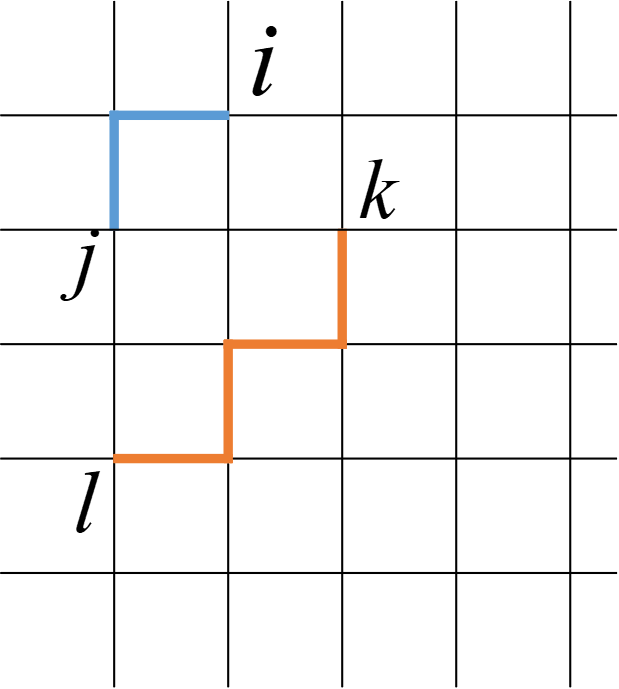
\includegraphics[width=3in]{Img/manhattan.png}
    \caption{Manhattan 距离的示意图。} 
\end{figure}
% 下面考虑 \eqref{Heff-taylor} 各项展开式中 $D$ 的阶数.
% \par $n=1$ 时: 
% \begin{equation}
%     -\sum_{i\ne o}\lag S_i \rag_oJ_{io}S_o\sim \frac{\tilde{J}_1}{D}D+\frac{\tilde{J}_2}{D^2}D^2+\cdots
% \end{equation}
可以证明, 当 $D\to \infty$ 时, 只有 $n=1$ 项保留, 高阶项为零。有效哈密顿量可以表示为
\begin{equation}
    \hoeff [S_o]= -h S_o-\sum_{i\ne o}J_{oi}\lag S_i \rag^{(o)}.
\end{equation}
从中可以定义有效场 $h_{\fun{eff}}$:
\begin{equation}
    h_{\fun{eff}}=h+\sum_{i\ne o}J_{oi}\lag S_i \rag^{(o)},\quad \hoeff =-h_{\fun{eff}}S_o.
\end{equation}
考虑到格点的平移不变性 $\lag S_o \rag=\lag S_i \rag$ 后, 这一结果与 Weiss 平均场理论一致。

\subsection{Hubbard model}
下面考虑量子情形。

Hubbard 模型的哈密顿量为
\begin{equation}
    \hat{H}=-\sum_{ij\sigma}t_{ij}^{ }c_{i\sigma}^\dg c_{j\sigma}^{ }+U\sum_i n_{i\ua} n_{i\da},
\end{equation}
其中, 设 $t_{ii}=0$, $t_{ij}=t_{ji}\in \mathbb{R}$。

在相干态路径积分下, 有配分函数 
\begin{equation}
    Z=\int\prod_{i}\prod_\sigma \mathcal{D}c_{i\sigma}^*(\tau)\mathcal{D}c_{j\sigma}^{ }(\tau)\e^{-S},
\end{equation}
其中作用量的表达式为
\begin{equation}
    S=\int_0^\infty\dd\tau\lmi \sum_{i\sigma}c_{i\sigma}^*(\tau)\ls \frac{\pt}{\pt \tau}-\mu \rs c_{i\sigma}(\tau)-\sum_{ij}\sum_\sigma t_{ij}c_{i\sigma}^*(\tau)c_{j\sigma}^{ }(\tau)+U\sum_i n_{i\ua}(\tau)n_{i\da}(\tau) \rmi,
\end{equation}
将作用量划分为空腔 $o$ 格点项 $S_o$, 剩余格点项 $S^{(o)}$ 以及相互作用项 $\Delta S$, 其中 
\begin{equation}
    S_o=\int_0^\beta\dd\tau\lmi \sum_\sigma c_{o\sigma}^*(\tau)\ls \frac{\pt}{\pt \tau}-\mu \rs c_{o\sigma}^{ }(\tau)+Un_{o\ua}(\tau)n_{o\da}(\tau) \rmi,
\end{equation}
\begin{equation}
    \Delta S=-\int_0^\beta \dd\tau\sum_{i\sigma}t_{io}\lmi c_{i\sigma}^*(\tau)c_{o\sigma}^{ }(\tau)+c_{o\sigma}^*(\tau)c_{i\sigma}^{ }(\tau) \rmi.
\end{equation}
记 $\eta_{i\sigma}(\tau)\equiv t_{io}c_{o\sigma}(\tau)$, 并对 $t_{ij}$ 作标度变换:
\begin{equation}
    t_{ij}=\frac{\tilde{t}_{ij}}{D^{\frac{|i-j|}{2}}}.
\end{equation}
这里的标度变换方式与 Ising 模型的处理不同, D. Vollhardt 证明, 这样的取法可以在大维度极限 $D\to \infty$ 时得到有限的 $\lag H_T \rag$, 否则将发散或趋于零\cite{PhysRevLett.62.324}。

定义空腔格点的有效作用量:
\begin{equation}
    \frac{1}{Z_{\fun{eff}}}\e^{-S_{\fun{eff}}}\equiv \frac{1}{Z}\int\prod_{i\ne o}\prod_{\sigma}\mathcal{D}c_{i\sigma}^*\mathcal{D}c_{i\sigma}^{ }\e^{-S},
\end{equation}
为方便表述, 令 $\eta_1^*,\cdots,\eta_{N}^*\equiv \eta_{N+1},\cdots,\eta_{2N}$, 视为和 $\eta_1,\cdots,\eta_{N}$ 相互独立的变量。利用 Grassmann 函数的泰勒展开式:
\begin{equation}
    \begin{aligned}
        S_{\fun{eff}}(\eta_{1},\cdots,\eta_{2N})=&\int\dd\tau L_{\fun{eff}}\\
        =&\int\dd\tau\sum_{n=0}^\infty\sum_{i_1\cdots i_n=1}^{2N}\frac{1}{n!}\left.\frac{\pt^n L_{\fun{eff}}}{\pt\eta_{i_1}\cdots\pt \eta_{i_n}}\right|_{\{\eta_1,\cdots,\eta_{2N}=0\}}\eta_{i_n}\cdots\eta_{i_1},
    \end{aligned}
\end{equation}
利用 
\begin{equation}
    \frac{\pt \eta_{i\sigma}(\tau)}{\pt \eta_{j\sigma'}(\tau')}=\delta_{ij}\delta_{\sigma\sigma'}\delta(\tau-\tau')
\end{equation}
以及有效作用量的定义式, 可以计算各阶偏导数的表达式:
\begin{equation}
    \begin{aligned}
        -\e^{-S_{\fun{eff}}}\int\dd\tau\frac{\pt L_{\fun{eff}}}{\pt \eta_{i_1\sigma}}&=\int\prod_{k\ne o}\prod_\sigma\mathcal{D}c_{k\sigma}^*\mathcal{D}c_{k\sigma}^{ }\e^{-S}\lmi -\int\dd\tau c_{i_1\sigma}^*\rmi\\
        \Rightarrow \int\dd\tau\lmi \e^{-S_{\fun{eff}}}\frac{\pt L_{\fun{eff}}}{\pt \eta_{i_1}} \rmi &=\int\dd\tau\lmi \int\prod_{k\ne o}\prod_\sigma\mathcal{D}c_{k\sigma}^*\mathcal{D}c_{k\sigma}^{ }\e^{-S} c_{i_1\sigma}^* \rmi,
    \end{aligned}
\end{equation}
从中得到 
\begin{equation}
    \begin{aligned}
        \left.\frac{\pt L_{\fun{eff}}}{\pt \eta_{i_1}}\right|_{\{\eta_{1,\cdots,N},\eta_{1,\cdots,N}^*=0\}}=&\frac{\int\prod_{k\ne o}\prod_{\sigma}\mathcal{D}c_{k\sigma}^*\mathcal{D} c_{k\sigma}^{ }\e^{-S^{(o)}}c_{i_1\sigma}^*}{\int\prod_{k\ne o}\prod_{\sigma}\mathcal{D}c_{k\sigma}^*\mathcal{D} c_{k\sigma}^{ }\e^{-S^{(o)}}}\\
        =&\lag c^*_{i_1\sigma}(\tau_{i_1}) \rag^{(o)},
    \end{aligned}
\end{equation}
但是奇数阶 Grassmann 变量的期望值都是 0, 所以这里得到的一阶导为零。再求一次导, 得到 
\begin{equation}
    \begin{aligned}
        \left.\frac{\pt^2 L_{\fun{eff}}}{\pt \eta_{i_1}^{ }\pt \eta_{j_1}^*}\right|_{\{\eta_{1,\cdots,N},\eta_{1,\cdots,N}^*=0\}}&=-\left.\frac{\pt^2 L_{\fun{eff}}}{\pt \eta_{i_1}^{*}\pt \eta_{j_1}^{ }}\right|_{\{\eta_{1,\cdots,N},\eta_{1,\cdots,N}^*=0\}}\\
        &=- \lag c_{j_1\sigma}^{ }(\tau_{j_1})c_{i_1\sigma}^*(\tau_{i_1}) \rag^{(o)}\\
        &=-G^{(o)}(\tau_{j_1},\tau_{i_1}).
    \end{aligned}
\end{equation}
同理, 应有
\begin{equation}
    \left.\frac{\pt^{2n}L_{\fun{eff}}}{\pt\eta_{j_1\sigma}^*\cdots\pt\eta_{j_n}^*\pt \eta_{i_1}^{ }\cdots\pt \eta_{i_n}^{ }}\right|_{\{\eta_{1,\cdots,N},\eta_{1,\cdots,N}^*=0\}}=(-1)^nG^{(o)}(\tau_{j_1}\cdots\tau_{j_n},\tau_{i_1}\cdots\tau_{i_n}).
\end{equation}
在 Taylor 展开式中, 首先, 只考虑 $\eta\eta^*$ 耦合, 不考虑 $\eta\eta$ 和 $\eta^*\eta$ 耦合, 其次, $2n$ 个 Grassmann 变量换序时会产生符号变化 $(-1)^n$ 与上式的符号抵消, 最后, 对应每一阶 $n$, 确定了 $i_1,\cdots,i_n,j_1,\cdots,j_n$ 的取值后, 应有 $n!$ 种排列组合方式, 写成正规形式后可以合并为一项。这样, 展开式可以表示为
\begin{equation}
    \begin{aligned}
        S_{\fun{eff}}=&\sum_{n=0}^\infty \sum_{\lag i_1,\cdots,i_n=1 \rag}^N\sum_{\lag j_1,\cdots,j_n=1 \rag}^N\int \left.\frac{\pt^{2n} L_{\fun{eff}}}{\pt \eta_{i_1}^{ }\cdots\pt\eta_{i_n}^{ }\pt \eta_{j_1}^*\cdots\pt\eta_{j_n}^*}\right|_{\{\eta_1^{ },\cdots,\eta_N^*=0\}}\eta_{j_n}^*\cdots\eta_{j_1}^*\eta_{i_n}\cdots\eta_{i_1}\\
        =&\sum_{n=1}^\infty \sum_{i_1\cdots j_n}\int\eta_{i_1}^*(\tau_{i_1})\cdots \eta_{i_n}^*(\tau_{i_n})\eta_{j_1}(\tau_{j_1})\cdots \eta_{j_n}(\tau_{j_n})G_{i_1\cdots j_n}^{(o)}(\tau_{i_1}\cdots \tau_{i_n},\tau_{j_1}\cdots \tau_{j_n})+S_o+\fun{const.}
    \end{aligned}
\end{equation} 
其中, 忽略了 $\eta_{i\sigma}(\tau)$ 的自旋指标和对 $\tau$ 的依赖关系。此即综述中 (34) 式。在大维度极限 $D\to \infty$ 下, 可以证明, 各阶展开中, 只有 $n=1$ 项保留下来, 其他高阶项快速衰减。于是有效作用量可以简化为 
 \begin{equation}
    S_{\fun{eff}}=S_o+\int_0^\beta\dd\tau\int_0^\beta\dd\tau'\sum_\sigma c_{i\sigma}^*(\tau)\lmi \sum_{ij}t_{oi}t_{oj}G_{ij}^{(o)}(\tau-\tau') \rmi c_{o\sigma}^{ }(\tau'),
 \end{equation}
中括号内的表达式被称为动力学平均场。整个积分式描写了周围格点对 $o$ 格点的影响。另外, $S_o$ 的表达式为 
\begin{equation}
    S_o=\int_0^\beta\dd\tau\sum_\sigma\lmi c_{o\sigma}^*(\tau)\ls \frac{\pt}{\pt \tau}-\mu \rs c_{o\sigma}^{ }(\tau) \rmi+\int_0^\beta\dd\tau\lmi U n_{o\ua}(\tau)n_{o\da}(\tau) \rmi.
\end{equation} 
由单杂质安德森模型 
\begin{equation}
    H_{\fun{SAIM}}=\epsilon_d\sum_\sigma d_\sigma^\dg d_\sigma^{ }+\sum_{k\sigma}\lmi \epsilon_k c_{k\sigma}^{\dg} c_{k\sigma}^{ }+V_k\ls d_\sigma^\dg c_{k\sigma}^{ }+c_{k\sigma}^\dg d_\sigma^{ } \rs \rmi+U n_{\ua}^d n_{\da}^d, 
\end{equation}
对应的杂质作用量为 
\begin{equation}
    S_{\fun{imp}}[d_\sigma^*,d_\sigma^{ }]=\int_0^\beta\dd\tau\int_0^\beta\dd\tau'd_\sigma^*(\tau)\lmi -\mathcal{G}^{-1}_0(\tau-\tau') \rmi d_{\sigma}(\tau')+U\int_0^\beta\dd\tau n_{\ua}^d(\tau)n_{\da}^d(\tau).
\end{equation}
上面得到的 $S_{\fun{eff}}$ 可以写成类似的形式, 即
\begin{equation}
    \begin{aligned}
        S_{\fun{eff}}=&\int_0^\beta\dd\tau \int_0^\beta\dd\tau'\sum_\sigma c_{o\sigma}^*(\tau)\lmi \ls \frac{\pt}{\pt \tau}-\mu \rs\delta(\tau-\tau')+\sum_{ij}t_{oi}t_{oj}G_{ij}^{(o)}(\tau-\tau') \rmi c_{o\sigma}(\tau')\\
        & +\int_0^\beta\dd\tau Un_{o\ua}(\tau)n_{o\da}(\tau)\\
        =&\int_0^\beta\dd\tau \int_0^\beta\dd\tau'\sum_\sigma c_{o\sigma}^*(\tau)\lmi \delta^{(1)}(\tau-\tau')-\mu\delta(\tau-\tau') +\sum_{ij}t_{oi}t_{oj}G_{ij}^{(o)}(\tau-\tau') \rmi c_{o\sigma}(\tau')\\
        &+\int_0^\beta\dd\tau Un_{o\ua}(\tau)n_{o\da}(\tau),
    \end{aligned}
\end{equation}
对比两式, 得到 
\begin{equation}
    \mathcal{G}_0^{-1}(\tau-\tau')=\delta^{(1)}(\tau-\tau')-\mu\delta(\tau-\tau') +\sum_{ij}t_{oi}t_{oj}G_{ij}^{(o)}(\tau-\tau'),
\end{equation}
变换到频率表象下, 有 
\begin{equation}
    \mathcal{G}_0 ^{-1}(\ii\omega_n)=\ii\omega_n+\mu-\sum_{ij}t_{oi}t_{oj}G_{ij}^{(o)}(\ii\omega_n).\label{weiss-eq}
\end{equation}
人们一般也将这里的无库仑相互作用格林函数 $\mathcal{G}_0$ 称为 Weiss 函数。这样就将晶格模型映射为了杂质模型。

在一般情况下,格点自能应该是动量依赖的,但在无穷维极限下,格点自能是对角的。在这种近似下,格点自能函数就等于空腔的自能函数,没有动量依赖\cite{Hartmann1989},即 
\begin{equation}
    \Sigma(\vct{k},\ii\omega_n)=\Sigma(\ii\omega_n)=\Sigma_{oo}(\ii\omega_n),
\end{equation}

为了自洽地将晶格模型映射到杂质模型,要求两个体系的格点可观测量和相互作用项都对应相等,也就是要求两个体系的自能函数相同,再利用上式,就得到杂质自能等于空腔自能,即 
\begin{equation}
    \Sigma_{\fun{imp}}(\ii\omega_n)=\Sigma_{oo}(\ii\omega_n).\label{dmftscf1}
\end{equation}
上式等价于
\begin{equation}
    G_{\fun{imp}}(\ii\omega_n)=G_{oo}(\ii\omega_n).\label{dmftscf2}
\end{equation}

利用杂质模型的 Dyson 方程,可以得到 
\begin{equation}
    G_{\fun{imp}}(\ii\omega_n)=\lb \mathcal{G}_0^{-1}(\ii\omega_n)-\Sigma_{\fun{imp}}(\ii\omega_n) \rb^{-1},\label{dmftscf3}
\end{equation}

另外,在 $D=\infty$ 极限下,晶格模型的格林函数具有下面的关系式\cite{PhysRevB.77.235106} 
\begin{equation}
    G_{ij}^{(o)}(\ii\omega_n)=G_{ij}(\ii\omega_n)-\frac{G_{io}(\ii\omega_n)G_{oj}(\ii\omega_n)}{G_{oo}(\ii\omega_n)},\label{lattice-G}
\end{equation}

以上四式已构成封闭方程组,为自洽求解,下面作进一步简化处理。

下面由式\eqref{lattice-G}出发,推导空腔电子格林函数对应的 Dyson 方程。首先引入格点格林函数的傅里叶变换形式为
\begin{equation}
    \sum_{ij}G_{ij}(\ii\omega_n)=\frac{1}{\mathcal{N}_s}\sum_{k}G_{k}(\ii\omega_n),
\end{equation}
其中 $\mathcal{N}_s$ 是格点数。

对式\eqref{lattice-G}两边同乘以 $t_{io}t_{oj}$ 并对 $i,j$ 求和,得到
\begin{equation}
    \begin{aligned}
        \sum_{ij}t_{io}t_{oj}G_{ij}^o(i\omega_n)=&\sum_{ij}t_{io}t_{oj}\lmi G_{ij}(i\omega_n)-\frac{G_{io}(\ii\omega_n)G_{oj}(\ii\omega_n)}{G_{oo}(\ii\omega_n)} \rmi\\
        =& \sum_{ij}t_{io}t_{oj}G_{ij}(\ii\omega_n)-\frac{\lmi \sum_i t_{io}G_{io}(\ii\omega_n) \rmi^2}{G_{oo}(\ii\omega_n)},
    \end{aligned}
\end{equation}
上式等号右边第一项经过傅里叶变换可以写成 
\begin{equation}
    \begin{aligned}
        \sum_{ij}t_{io}t_{oj}G_{ij}(\ii\omega_n)=& \frac{1}{\mathcal{N}_s}\sum_k\epsilon_k^2G_k(\ii\omega_n)\\
        =&\frac{1}{\mathcal{N}_s}\sum_k\epsilon_k^2\lmi \ii\omega_n +\mu-\epsilon_k-\Sigma_{oo}(\ii\omega_n) \rmi^{-1}\\
        \equiv & \frac{1}{\mathcal{N}_s}\sum_k\frac{\epsilon_k^2}{\xi -\epsilon_k}\\
        \equiv & \int\dd \epsilon D(\epsilon)\frac{\epsilon^2}{\xi -\epsilon},
    \end{aligned}
\end{equation}
其中第三步定义了
\begin{equation}
    \xi\equiv \ii\omega_n+\mu-\Sigma_{oo}(\ii\omega_n),\label{equiv-freq}
\end{equation}
第四步的晶格态密度定义为 
\begin{equation}
    D(\epsilon)\equiv \frac{1}{\mathcal{N}_s}\sum_{k}\delta(\epsilon-\epsilon_k).
\end{equation}
类似地有第二项的傅里叶变换
\begin{equation}
    \begin{aligned}
        \frac{\lmi \sum_i t_{io}G_{io}(\ii\omega_n) \rmi^2}{G_{oo}(\ii\omega_n)}=&\frac{\lmi \frac{1}{\mathcal{N}_s}\sum_k\frac{\epsilon_k}{\xi-\epsilon_k} \rmi^2}{(\xi-\epsilon_k)^{-1}}\\
        =& \frac{\lmi \int\dd\epsilon D(\epsilon)\frac{\epsilon}{\xi-\epsilon} \rmi^2}{\int\dd\epsilon D(\epsilon)\frac{1}{\xi-\epsilon}}.
    \end{aligned}
\end{equation}
考虑恒等关系 
\begin{equation}
    \int\dd\epsilon D(\epsilon)\frac{\epsilon}{\xi-\epsilon}=-1+\xi\int\dd\epsilon\frac{D(\epsilon)}{\xi-\epsilon},\label{equiv1}
\end{equation}
以及 
\begin{equation}
    \begin{aligned}
        \int\dd\epsilon D(\epsilon)\frac{\epsilon^2}{\xi-\epsilon}=& \int\dd\epsilon D(\epsilon)\epsilon \ls -1+\frac{\xi}{\xi-\epsilon} \rs\\
        =&-\int\dd\epsilon D(\epsilon)\epsilon +\xi\int\dd\epsilon D(\epsilon)\frac{\epsilon}{\xi-\epsilon}\\
        =&\xi\int\dd\epsilon D(\epsilon)\frac{\epsilon}{\xi-\epsilon},
    \end{aligned}\label{equiv2}
\end{equation}
其中最后一步利用了空腔格点的傅里叶变换关系 $\int D(\epsilon)\epsilon=\sum_kt_k=t_{oo}=0$.

利用\eqref{equiv1}和\eqref{equiv2},空腔电子格林函数的格林函数可以写成
\begin{equation}
    \begin{aligned}
        \sum_{ij}t_{io}t_{oj}G_{ij}^{(o)(\ii\omega_n)}=& \xi\int\dd\epsilon D(\epsilon)\frac{\epsilon}{\xi-\epsilon}=\frac{\lmi -1+\xi\int\dd\epsilon \frac{D(\epsilon)}{\xi-\epsilon} \rmi^2}{\int\dd\epsilon D(\epsilon)\frac{1}{\xi-\epsilon}}\\
        =& \xi\int\dd\epsilon D(\epsilon)\frac{\epsilon}{\xi-\epsilon}-\frac{1-\int\dd\epsilon D(\epsilon)\frac{2\xi}{\xi-\epsilon}+\int\dd\epsilon D(\epsilon)\frac{\xi^2}{\xi-\epsilon}}{\int\dd\epsilon D(\epsilon)\frac{1}{\xi-\epsilon}}\\
        =& \xi\int\dd\epsilon D(\epsilon)\frac{\epsilon}{\xi-\epsilon} -\lmi \int\dd\epsilon D(\epsilon)\frac{1}{\xi-\epsilon} \rmi^{-1} \\
        &+2\xi-\xi^2 \int\dd\epsilon D(\epsilon)\frac{1}{\xi-\epsilon}\\
        =& -\lmi \xi\int\dd\epsilon D(\epsilon)\frac{1}{\xi-\epsilon} \rmi^{-1}+\xi,
    \end{aligned}
\end{equation}
将上式代入到 Weiss 函数的表达式\eqref{weiss-eq}中,并利用\eqref{equiv-freq}和空腔格林函数的傅里叶变换,就得到了空腔电子格林函数的 Dyson 方程 
\begin{equation}
    \mathcal{G}_0^{-1}(\ii\omega_n)=\Sigma_{oo}(\ii\omega_n)+G_{oo}^{-1}(\ii\omega_n).\label{dmftscf4}
\end{equation}
综合上述推导,\eqref{dmftscf1} \eqref{dmftscf2} \eqref{dmftscf3}和\eqref{dmftscf4} 构成了动力学平均场理论的自洽方程组:
\begin{equation}
    \begin{aligned}
        & \fun{(a)}\quad \Sigma_{\fun{imp}}(\ii\omega_n)=\Sigma_{oo}(\ii\omega_n),\\
        & \fun{(b)}\quad G_{\fun{imp}}(\ii\omega_n)=G_{o}(\ii\omega_n),\\
        & \fun{(c)}\quad G^{-1}_{\fun{imp}}(\ii\omega_n)=\mathcal{G}_0^{-1}(\ii\omega_n)-\Sigma_{\fun{imp}}(\ii\omega_n),\\
        & \fun{(d)}\quad \Sigma_{oo}(\ii\omega_n)=\mathcal{G}_0^{-1}(\ii\omega_n)+G_{oo}^{-1}(\ii\omega_n).
    \end{aligned}
\end{equation}
这样,动力学平均场理论就将晶格模型映射到了单杂质模型中,问题转化成了对杂质模型的求解。在前面得到的自洽方程组中,人们需要自洽地求出 $G_{\fun{imp}}$ 和 $\mathcal{G}_0$。实际处理问题时,通常的方法是先猜测一个 $\mathcal{G}_0$ 初值,通过杂质求解器计算得到 $G_{\fun{imp}}$ 和 $\Sigma_{\fun{imp}}$,然后利用 DMFT 自洽条件得到新的 $\mathcal{G}_0$,重复这一迭代过程直到 $(G_{\fun{imp}},\mathcal{G}_0)$ 同时收敛。

在迭代过程中,最重要的步骤是对杂质模型的求解。虽然在无穷维极限下人们已经冻结了模型的空间涨落,但是杂质模型仍然是一个严格的多体问题。对于这一问题,早在 DMFT 发展之前几十年,人们就已经发展出了许多杂质模型的求解技术,可以直接迁移到 DMFT 计算中去。不同的杂质求解器适用范围和优势各有不同,它们的精度和效率直接决定着 DMFT 方法的求解性能。在 eDMFT 程序中常使用的是连续时间量子蒙特卡洛方法作为杂质求解器\cite{RevModPhys.83.349},由于这一方法计算效率高,适用范围广,因此它的出现迅速取代了之前的一些量子蒙特卡洛方法(如 Hirsch-Fye 算法\cite{PhysRevLett.56.2521},CT-INT 算法\cite{PhysRevB.72.035122}等等),成为目前应用最广泛的杂质求解器之一。
\section{量子杂质模型求解器}
对杂质模型的求解,按不同的求解方案,一般可以分为精确解、解析近似求解和数值求解。然而,精确的 Bethe ansatz 只能严格求解具有特殊形式杂化函数的单杂质安德森模型,无法应用到 DMFT 框架中。因此人们只能使用各种解析方法和数值方法近似求解。解析方法中,一类重要方法是图形展开。这种方法的重要代表是非交叉近似(Non-crossing Approximation, NCA)\cite{RevModPhys.59.845}和单交叉近似(One-crossing Approximation, OCA)\cite{PhysRevB.64.155111},做法是对杂化项作费曼图展开,保留所有直线没有相交的图即为 NCA 方法,保留直线只交叉一次的即 OCA 方法,两种程度的近似分别对应着杂化函数的二阶和四阶微扰展开。

与解析近似方法相比,数值方法是一类相对更强大的方法,这一类方法的误差来自于参数离散化或抽样引入的系统误差,因此原则上只要耗费足够多的计算资源,就能够得到相当高精度的结果。在强关联电子体系中,近年来使用较广泛的一种数值求解方法是基于强耦合展开的连续时间量子蒙特卡洛方法(CT-HYB),原则上这种数值方法能够对所有阶展开图进行抽样,这是与半解析的 NCA 或 OCA 方法的一个区别\cite{PhysRevLett.97.076405}。下面从蒙特卡洛的基本原理出发,对这一方法作简要介绍。
\subsection{蒙特卡洛方法}
蒙特卡洛(Monte Carlo)方法是一种基于概率和统计的计算方法,核心思想是对统计系综下的物理量进行抽样计算。依照这一思想,物理体系的配分函数可以写成对位形空间中所有位形 $x$ 按权重 $p(x)$ 积分的形式,即
\begin{equation}
    \mathcal{Z}=\int_{\fun{C}}\dd x p(x),
\end{equation}
对物理量 $A$ 期望值的计算也可以相应地写成 
\begin{equation}
    \lag A\rag =\frac{1}{\mathcal{Z}}\int_{\fun{C}}\dd x A(x)p(x),
\end{equation}
其中 $\fun{C}$ 表示对整个位形空间作积分。对于经典系统而言,每个构型对应的权重为 
\begin{equation}
    p(x)=\exp\ls -\beta E(x) \rs,
\end{equation}
对量子系统而言,位形空间中的每一项都与配分函数展开的各阶费曼图一一对应。蒙特卡洛的抽样思路是抽取 $M$ 个位形 $x_i$,物理量 $\lag A\rag$ 就可以近似表示为 
\begin{equation}
    \lag A \rag\approx \lag A\rag_{\fun{MC}}\equiv \frac{1}{M}\sum_{i=1}^M A(x_i),
\end{equation}
当抽样足够多时,方便起见,人们也常将表达式改写为 
\begin{equation}
    \begin{aligned}
        \lag A \rag = & \frac{1}{\mathcal{Z}} \int_{\fun{C}}\dd x A(x)p(x)\\
        \equiv & \frac{\int_{\fun{C}}\dd x A(x)\frac{P(x)}{\rho(x)}\rho(x)}{\int_{\fun{C}}\dd x \frac{P(x)}{\rho(x)}\rho(x)}\\
        =&\frac{\llag A\frac{P}{\rho} \rrag_\rho}{\llag \frac{P}{\rho} \rrag_\rho}.
    \end{aligned}
\end{equation}
一般人们利用马尔可夫过程(Markov process)来产生足够多的位形。假设有相空间中的位形 $x,y,z,\cdots$,考虑如下形式的马尔可夫链 
\begin{equation}
    x\to y\to z\to \cdots,
\end{equation}
定义由 $x$ 位形直接跳跃到 $y$ 位形的概率为 $W_{xy}$,那么应有 
\begin{equation}
    \sum_{y\in \fun{C}} W_{xy}=1,
\end{equation}
即由任意位形出发,跳跃到其他任意状态的概率之和恒为 $1$。为了利用马尔可夫过程,从任意初态出发,快速演化到某一特定分布状态,需要满足两个充分条件:
\begin{itemize}
    \item[1] \textbf{各态历经(Ergodicity)}从任意位形 $x$ 出发,总可以由有限个马尔可夫过程到达任意位形 $y$,即 
    \begin{equation}
        \forall x, y \in \fun{C},\ \exists N<\infty,\ \fun{i. e.}\ \forall n\ge N,\ (W^n)_{xy}\ne 0.
    \end{equation}
    \item[2] \textbf{细致平衡条件(Detailed balance condition)}从某一位形 $x$ 出发到达另一位形 $y$ 的概率密度,应与从 $y$ 出发到达 $x$ 的概率密度相等,即 
    \begin{equation}
        \frac{W_{xy}}{W_{yx}}=\frac{p(y)}{p(x)}.
    \end{equation}
\end{itemize}
为了产生满足以上要求的马尔可夫链,人们通常采用的是 Metropolis-Hastings 算法\cite{Hastings1970MonteCS, 1953JChPh..21.1087M}。在这一算法中,人们假定状态 $x$ 跳跃到 $y$ 的概率 $W_{xy}$ 由两部分构成,即 
\begin{equation}
    W_{xy}=W_{xy}^{\fun{prop}}W_{xy}^{\fun{acc}},
\end{equation}
其中 $W_{xy}^{\fun{prop}}$ 是 $x$ 可能向 $y$ 发生跳变的概率,$W_{xy}^{\fun{acc}}$ 是这一跳变过程被接收的概率。如果这一过程被接受,那么位形变成 $y$;如果不被接受,位形保持为 $x$、

利用前面给出的细致平衡条件公式,可以得到 
\begin{equation}
    \frac{W_{xy}^{\fun{acc}}}{W_{yx}^{\fun{acc}}}=\frac{p(y)W_{yx}^{\fun{prop}}}{p(x)W_{xy}^{\fun{prop}}}\equiv R,
\end{equation}
设 $W_{xy}^{\fun{acc}}$ 是关于 $R$ 的函数,即 
\begin{equation}
    W_{xy}^{\fun{acc}}=f\ls \frac{p(y)W_{yx}^{\fun{prop}}}{p(x)W_{xy}^{\fun{prop}}} \rs=f(R),
\end{equation}
相应地有 
\begin{equation}
    W_{yx}^{\fun{acc}}=f\ls \frac{p(x)W_{xy}^{\fun{prop}}}{p(y)W_{yx}^{\fun{prop}}} \rs =f(1/R).
\end{equation}
这样,细致平衡条件在形式上可以转化为以下条件:
\begin{equation}
    \frac{f(R)}{f(1/R)}=R.
\end{equation}
这一条件可以利用 Metropolis-Hastings 给出的函数形式来满足:
\begin{equation}
    f(R)=\min [1,R].
\end{equation}
\subsection{强耦合展开连续时间量子蒙特卡洛(CT-HYB)}
量子蒙特卡洛方法的基本思路是利用随机抽样方法求解量子力学问题,这一方法大致可以分为三类:变分蒙特卡洛(Variational Monte Carlo, VMC),路径积分蒙特卡洛(Path Integral Monte Carlo, PIMC)和辅助场蒙特卡洛(Auxiliary Field Monte Carlo, AFMC)。VMC 是在变分法的框架下对 Metropolis 方法的推广,这一方法的求解重点是相互作用多体系统的基态能和波函数;PIMC 的思路是对多体系统的作用量进行随机抽样;AFMC 方法的思路是将作用量离散化之后,将配分函数积分写成在位形空间中的求和,然后利用蒙特卡洛方法进行抽样计算。在实际强关联材料计算中,人们最常使用的连续时间量子蒙特卡洛算法就属于一种 PIMC 算法。下面具体介绍在强关联材料计算中使用的强耦合展开连续时间量子蒙特卡洛方法的原理和计算框架。

将模型哈密顿量拆分成无相互作用的 $H_0$ 和 $H_1$ 两部分,即
\begin{equation}
    H=H_0+H_1,
\end{equation}
相互作用表象下的时间演化算符可以表示为
\begin{equation}
    U(\tau)=\e^{H_0\tau}\e^{-H\tau},
\end{equation}
相应的含时算符 $O(\tau)$ 可以表示为
\begin{equation}
    O(\tau)=\e^{\tau H_1}O\e^{-\tau H_1}.
\end{equation}
时间演化算符对虚时 $\tau$ 求导可以得到 
\begin{equation}
    \begin{aligned}
        \frac{\dd U(\tau)}{\dd\tau}=& \e^{H_0\tau}(H_0-H)\e^{-H\tau}\\
        =& -\e^{H_0\tau} H_1 \e^{-H_0\tau}\e^{H_0\tau}\e^{H\tau}\\
        =&-H_1(\tau)U(\tau),
    \end{aligned}
\end{equation}
可以得到 $U(\tau)$ 的形式解 
\begin{equation}
    U(\tau)=T_{\tau}\exp\lmi -\int_0^{\tau}H_1(\tau')\dd\tau' \rmi.
\end{equation}
这样,就可以将体系的配分函数用含时演化算符表示出来之后,写成级数展开的形式
\begin{equation}
    \begin{aligned}
        \mathcal{Z}=&\fun{Tr}\lmi \e^{-\beta H} \rmi\\
        =& \fun{Tr}\lmi \e^{-\beta H_0}\fun{T}_{\tau}\exp\ls -\int_0^\beta H_1(\tau)\dd\tau \rs \rmi\\
        =& \sum_k\int_0^\beta \dd\tau_1\cdots\int_0^\beta \dd\tau_k\frac{(-1)^k}{k!}\fun{Tr}\lmi \e^{-\beta H_0}\fun{T}_{\tau}\ls H_1(\tau_k)\cdots H_1(\tau_1) \rs \rmi\\
        =& \sum_k\int_0^\beta \dd\tau_1\cdots \int_{\tau_{k-1}}^\beta \dd\tau_{k}(-1)^k \fun{Tr}\lmi \e^{-\beta H_0}H_1(\tau_k)\cdots H_1(\tau_1) \rmi.
    \end{aligned}\label{cthyb-Z}
\end{equation}
接下来就可以使用蒙特卡洛抽样方法来处理这一级数求和表达式。在这一级数展开式中,并没有对虚时间 $\tau$ 作离散化处理,因此人们称这一展开方式为连续时间量子蒙特卡洛方法。

将前面给出的单杂质安德森模型重新写成以下形式 
\begin{equation}
    H_{\fun{SIAM}}=H_{\fun{loc}}+H_{\fun{bath}}+H_{\fun{hyb}},
\end{equation}
在杂化项展开的抽样方法中,哈密顿量的前两项取为 $H_0$,即 
\begin{equation}
    \begin{aligned}
        H_0\equiv& H_{\fun{loc}}+H_{\fun{bath}}\\
        =& \underbrace{\epsilon_d\sum_{\sigma}d_\sigma^\dg d_\sigma+U n_{\ua}^d n_{\da}^d}_{H_{\fun{loc}}}+\underbrace{\sum_{k\sigma}\epsilon_k c_{k\sigma}^\dg c_{k\sigma}}_{H_{\fun{bath}}},
    \end{aligned}
\end{equation}
杂化项取为作微扰展开的 $H_1$,即 
\begin{equation}
    H_1\equiv H_{\fun{hyb}}=\underbrace{\sum_{k\sigma}V_k d_\sigma^\dg c_{k\sigma}^{ }}_{\tilde{H}_{\fun{hyb}}}+\underbrace{\sum_{k\sigma}V_k^* c_{k\sigma}^\dg d_\sigma^{ }}_{\tilde{H}_{\fun{hyb}}^\dg}.
\end{equation}
由于强耦合展开需要考虑对杂化项的各阶乘积求迹,这里杂化项的每一项只有一个 $d$ 电子算符和一个 $c$ 电子算符,因此在求迹时,只有偶数个 $H_{\fun{hyb}}$ 相乘的项不为零。其中每 $2n$ 个 $H_{\fun{hyb}}$ 相乘时,只有 $\fun{C}_{2n}^n=\left. (2n)!\right/(n!n!)$ 个 $\lmi \tilde{H}_{\fun{hyb}}\tilde{H}_{\fun{hyb}}^\dg \rmi^n$ 保留下来。将模型哈密顿量的具体表达式代入到式 \eqref{cthyb-Z} 给出的配分函数中,单杂质安德森模型可以表示为 
\begin{equation}
    \begin{aligned}
        \mathcal{Z}=& \sum_{nn'} \int_0^\beta \dd\tau_1\cdots \int_0^\beta \dd\tau_n \int_0^\beta\dd\tau_{1'}\cdots \int_0^\beta \dd\tau_{n'}\\
        &\times \frac{1}{(2n)!} \fun{Tr}\lmi \e^{-\beta H_0} \frac{(2n)!}{n!n!}\fun{T}_{\tau}\ls \tilde{H}_{\fun{hyb}}(\tau_n)\tilde{H}_{\fun{hyb}}^\dg (\tau_{n'})\cdots \tilde{H}_{\fun{hyb}(\tau_1)}\tilde{H}_{\fun{hyb}}^\dg (\tau_{1'}) \rs \rmi\\
        =&\sum_{nn'}\int_0^\beta \dd\tau_1\cdots\int_{\tau_{n-1}}^\beta\dd\tau_n\int_0^\beta \dd\tau_{1'}\cdots\int_{\tau_{n'-1}}^\beta\dd\tau_{n'}\\
        &\times V_{k_n}^{ }V_{k_{n'}}^* V_{k_{n-1}}^{ }V_{k_{n'-1}}^*\cdots V_{k_1}^{ }V_{k_{1'}}^*\\
        & \times\fun{Tr}\lmi \e^{-\beta H_0}\ls c_{k_n\sigma_n}(\tau_n)d_{\sigma_n}(\tau_n)d_{\sigma_{n'}}^\dg(\tau_{n'})c_{k_{n'}\sigma_{n'}}(\tau_{n'})\times \cdots \right.\right. \\
        & \qquad\qquad\quad\quad \left.\left. \times c_{k_1\sigma_1}^\dg(\tau_1)d_{\sigma_1}(\tau_1)d_{\sigma_{1'}}^\dg (\tau_{1'})c_{k_{1'}\sigma_{1'}}(\tau_{1'}) \rs \rmi,
    \end{aligned}
\end{equation}
将配分函数中的 $c$ 电子项和 $d$ 电子项拆分开,可以得到 
\begin{equation}
    \begin{aligned}
        \mathcal{Z}=&\sum_{nn'}\int_0^\beta \dd\tau_1\cdots \int_0^\beta \dd\tau_n \int_0^\beta\dd\tau_{1'}\cdots \int_0^\beta \dd\tau_{n'}\ls V_{k_n}^{ }V_{k_{n'}}^* V_{k_{n-1}}^{ }V_{k_{n'-1}}^*\cdots V_{k_1}^{ }V_{k_{1'}}^*\rs\\
        & \times\fun{Tr}_d\lmi \e^{-\beta H_{\fun{loc}}}\fun{T}_\tau \ls d_{\sigma_n}(\tau_n)d_{\sigma_{n'}}^\dg (\tau_{n'})\cdots d_{\sigma_1}(\tau_1)d_{\sigma_{1'}}^\dg(\tau_{1'}) \rs \rmi\\
        &\times \fun{Tr}_c\lmi \e^{-\beta H_{\fun{bath}}}\fun{T}_\tau \ls c_{k_n\sigma_n}^\dg (\tau_n) c_{k_{n'}\sigma_{n'}}(\tau_{n'})\cdots c_{k_1\sigma_1}^\dg (\tau_1)c_{k_{1'}\sigma_{1'}}(\tau_{1'}) \rs \rmi,
    \end{aligned}
\end{equation}
如果定义 bath 的配分函数为 
\begin{equation}
    \begin{aligned}
        \mathcal{Z}_{\fun{bath}}\equiv &\fun{Tr}\e^{-\beta H_{\fun{bath}}}\\
        =&\fun{Tr}\prod_{k\sigma}\ls 1-\beta\epsilon_kc_{k\sigma}^\dg c_{k\sigma}^{ }+\frac{1}{2!}(-\beta\epsilon_k)^2(c_{k\sigma}^\dg c_{k\sigma}^{ })^2+\cdots \rs,
    \end{aligned}
\end{equation}
其中 $c$ 电子算符的高阶乘积可以写成 
\begin{equation}
    c_{k\sigma}^\dg c_{k\sigma}^{ }c_{k\sigma}^\dg c_{k\sigma}=c_{k\sigma}^\dg c_{k\sigma}^{ }-c_{k\sigma}^{\dg} c_{k\sigma}^\dg c_{k\sigma}^{ }c_{k\sigma}^{ },
\end{equation}
在 $c$ 电子的单粒子基下求迹可以表示为 $\fun{Tr}(\cdots)=\lag 0|\cdots|0\rag +\lag 1|\cdots |1\rag$,因此高阶项求迹之后都是零,只有二阶项保留。这样 bath 配分函数可以简化为 
\begin{equation}
    \begin{aligned}
        \mathcal{Z}_{\fun{bath}}=& \fun{Tr}\prod_{k\sigma}\lmi 1+c_{k\sigma}^\dg c_{k\sigma}^{ }\ls -\beta \epsilon_k+\frac{(-\beta\epsilon_k)^2}{2!}+\cdots \rs \rmi\\
        =& \fun{Tr}\prod_{k\sigma}\lmi 1+c_{k\sigma}^\dg c_{k\sigma}^{ }\ls \e^{-\beta\epsilon_k}-1 \rs \rmi\\
        =&\prod_{k\sigma}\lb \llag 0\left| \lmi 1+c_{k\sigma}^\dg c_{k\sigma}^{ }(\e^{-\beta\epsilon_k}-1) \rmi \right| 0 \rrag + \llag 1 \left| \lmi 1+c_{k\sigma}^\dg c_{k\sigma}(\e^{-\beta\epsilon_k}-1) \rmi \right| 1 \rrag \rb\\
        =& \prod_{k\sigma}\ls 1+\e^{-\beta \epsilon_k} \rs,
    \end{aligned}
\end{equation}
相应地可以定义算符期望值 
\begin{equation}
    \lag\cdots\rag_0\equiv \frac{1}{\mathcal{Z}_{\fun{bath}}}\fun{Tr}_c\lmi \e^{-\beta H_{\fun{bath}}}\cdots \rmi.
\end{equation}
借助以上这些定义,体系总的配分函数中,与 $c$ 电子有关的部分可以表示成 
\begin{equation}
    \begin{aligned}
        &V_{k_n}V_{k_{n'}}^*\cdots V_{k_1}V_{k_{1'}}^*\fun{Tr}_c \lmi \e^{-\beta H_{\fun{bath}}}\fun{T}_\tau \ls c_{k_n\sigma_n}^\dg(\tau_n)c_{k_{n'}\sigma_{n'}}(\tau_{n'})\cdots c_{k_1\sigma_1}^\dg(\tau_1)c_{k_{1'}\sigma_{1'}}(\tau_{1'}) \rs \rmi\\
        =&\mathcal{Z}_{\fun{bath}}\llag V_{k_n}V_{k_{n'}}^*\cdots V_{k_1}V_{k_{1'}}^* \fun{T}_{\tau}\ls c_{k_n\sigma_n}^\dg(\tau_n)c_{k_{n'}\sigma_{n'}}(\tau_{n'})\cdots c_{k_1\sigma_1}^\dg (\tau_1)c_{k_{1'}\sigma_{1'}}(\tau_{1'}) \rs \rrag_0.
    \end{aligned}
    \label{trace-c}
\end{equation}
上式中的编时算符乘积可以利用 Wick 定理进一步简化。不失一般性,选择其中两项缩并: 
\begin{equation}
    \begin{aligned}
        &\llag\ls V_{k_n}c_{\sigma_n k_n}^\dg (\tau_n) \rs \ls V_{k_{n'}}^* c_{\sigma_{n'}k_{n'}}(\tau_{n'}) \rs\rrag_0\\
        =& V_{k_n}V_{k_{n'}}^*\llag c_{\sigma_nk_n}^\dg (\tau_n)c_{\sigma_{n'}k_{n'}}(\tau_{n'}) \rrag_0\\
        =& V_{k_n}V_{k_{n'}}^*\frac{1}{\mathcal{Z}_{\fun{bath}}}\fun{Tr}_c\lmi \e^{-\beta H_{\fun{bath}}}\fun{T}_\tau \ls c_{\sigma_n k_\sigma}^\dg (\tau_n) c_{\sigma_{n'}k_{n'}}(\tau_{n'}) \rs \rmi,
    \end{aligned}
\end{equation}
分成两种情况考虑以上编时乘积。当 $\tau_n>\tau_{n'}$ 时,上式的求迹部分可以改写为
\begin{equation}
    \begin{aligned}
        &\fun{Tr}_c \lmi \e^{-\beta H_{\fun{bath}}}\e^{(H_{\fun{bath}}+H_{\fun{loc}})\tau_n}c_{\sigma_n k_n}^\dg \e^{-(H_{\fun{bath}}+H_{\fun{loc}})\tau_n}\e^{(H_{\fun{bath}+H_{\fun{loc}}})\tau_{n'}}c_{\sigma_{n'}k_{n'}}\e^{-(H_{\fun{bath}}+H_{\fun{loc}})\tau_{n'}} \rmi\\
        =& \fun{Tr}_c\lmi \e^{H_{\fun{bath}}(-\beta+\tau_n-\tau_{n'})}\e^{H_{\fun{loc}}(\tau_n-\tau_{n'})}c_{\sigma_nk_{n}}^\dg \e^{-H_{\fun{bath}}(\tau_k-\tau_{k'})}\e^{-H_{\fun{loc}}(\tau_n-\tau_{n'})}c_{\sigma_{n'}k_{n'}} \rmi\\
        =&  \fun{Tr}_c\lmi \e^{H_{\fun{bath}}(-\beta+\tau_n-\tau_{n'})}c_{\sigma_nk_n}^\dg \e^{-H_{\fun{bath}}(\tau_n-\tau_{n'})}c_{\sigma_{n'}k_{n'}} \rmi\\
        =&\delta_{\sigma_n\sigma_{n'}}\delta_{k_nk_{n'}}\llag 1_{\sigma_nk_n} \left| \fun{Tr}_{c}'\lmi \e^{H_{\fun{bath}}(-\beta+\tau_k-\tau_{k'})}c_{\sigma_nk_n}^\dg \e^{-H_{\fun{bath}}(\tau_k-\tau_{k'})}c_{\sigma_nk_n} \rmi \right| 1_{\sigma_nk_n}  \rrag\\
        =& \delta_{\sigma_n\sigma_{n'}}\delta_{k_nk_{n'}}\e^{\epsilon_{k_n}(-\beta+\tau_n-\tau_{n'})}\llag 0_{\sigma_nk_n}\left| \e^{-H_{\fun{bath}}(\tau_n-\tau_{n'})} \right| 0_{\sigma_n k_n} \rrag\times \fun{Tr}_c\lmi\prod_{m\ne n}\e^{-\beta\epsilon_{k_m}n_{\sigma_mk_m}}\rmi \\
        =& \delta_{\sigma_n\sigma_{n'}}\delta_{k_nk_{n'}}\e^{\epsilon_{k_n}(-\beta+\tau_n-\tau_{n'})}\fun{Tr}_c\lmi\prod_{m\ne n}\e^{-\beta\epsilon_{k_m}n_{\sigma_mk_m}}\rmi,
    \end{aligned}
\end{equation}
其中倒数第三步的求迹是对所有 $\sigma\ne \sigma_n$ 和 $k\ne k_n$ 进行的。将上式带回缩并式,就得到了 
\begin{equation}
    \begin{aligned}
        &\llag\ls V_{k_n}c_{\sigma_n k_n}^\dg (\tau_n) \rs \ls V_{k_{n'}}^* c_{\sigma_{n'}k_{n'}}(\tau_{n'}) \rs\rrag_0\\
        =&V_{k_n}V_{k_{n'}}^*\frac{1}{\mathcal{Z}_{\fun{bath}}}\delta_{\sigma_n\sigma_{n'}}\delta_{k_nk_{n'}}\e^{\epsilon_{k_n}(-\beta+\tau_n-\tau_{n'})}\fun{Tr}_c\lmi\prod_{m\ne n}\e^{-\beta\epsilon_{k_m}n_{\sigma_mk_m}}\rmi\\
        =&\delta_{\sigma_n\sigma_{n'}}\delta_{k_nk_{n'}}\frac{V_{k_n}V_{k_{n'}}^*}{1+\e^{-\beta\epsilon_n}}\e^{\epsilon_{k_n}(-\beta+\tau_n-\tau_{n'})}.
    \end{aligned}
\end{equation}
类似地,当 $\tau_n<\tau_{n'}$ 时,可以得到
\begin{equation}
    \llag\ls V_{k_n}c_{\sigma_n k_n}^\dg (\tau_n) \rs \ls V_{k_{n'}}^* c_{\sigma_{n'}k_{n'}}(\tau_{n'}) \rs\rrag_0=-\delta_{\sigma_n\sigma_{n'}}\delta_{k_nk_{n'}}\frac{V_{k_n}V_{k_{n'}}^*}{1+\e^{-\beta\epsilon_n}}\e^{\epsilon_{k_n}(\tau_n-\tau_{n'})}.
\end{equation}
这样,\eqref{trace-c} 按 Wick 定理的一种展开式就可以写成下面的形式:
\begin{equation}
    \sum_{\sigma_n}\sum_{k_n}\frac{V_{k_n}V_{k_{n'}}^*}{1+\e^{-\beta \epsilon_{k_n}}}\left\{
        \begin{aligned}
            &\e^{\epsilon_{k_n}(\tau_n-\tau_{n'}-\beta)},\quad \tau_n>\tau_{n'},\\
            &-\e^{\epsilon_{k_n}(\tau_n-\tau_{n'})},\quad \tau_n<\tau_{n'}.
        \end{aligned}
    \right.
\end{equation}
定义满足反周期性的杂化函数: 
\begin{equation}
    \Delta_{n'n}(\tau_n-\tau_{n'})\equiv\sum_{\sigma_n}\sum_{k_n}\frac{V_{k_n}V_{k_{n'}}^*}{1+\e^{-\beta \epsilon_{k_n}}}\left\{
        \begin{aligned}
            &\e^{\epsilon_{k_n}(\tau_n-\tau_{n'}-\beta)},\quad \tau_n>\tau_{n'},\\
            &-\e^{\epsilon_{k_n}(\tau_n-\tau_{n'})},\quad \tau_n<\tau_{n'}.
        \end{aligned}
    \right.
\end{equation}
可以把所有阶数 $n$ 和 $n'$ 不同的杂化函数统一写成一个矩阵 $\vct{M}^{-1}$,具体形式为 
\begin{equation}
    \vct{M}^{-1}\equiv 
    \left(
        \begin{aligned}
            &\Delta_{1'1}(\tau_1-\tau_{1'})\quad&\Delta_{2'1}(\tau_1-\tau_{2'})&\quad\cdots &\Delta_{N'1}(\tau_1-\tau_{N'})\\
            &\Delta_{1'2}(\tau_2-\tau_{1'})&\ddots&&\vdots\quad\\
            &\quad\vdots&\ddots&&\vdots\quad\\
            &\Delta_{1'N}(\tau_N-\tau_{1'})&\cdots &\cdots &\Delta_{N'N}(\tau_N-\tau_{N'})
        \end{aligned}
    \right),
\end{equation}
按照上述定义,配分函数中由费米子反对易关系带来的符号就可以吸收进 $\vct{M}^{-1}$ 的行列式中。最后,就得到了配分函数按杂化项展开的一般表达式: 
\begin{equation}
    \begin{aligned}
        \mathcal{Z}=&\sum_{nn'}\int_{0}^\beta \dd\tau_1\cdots\int_{\tau_{n-1}}^\beta \dd\tau_n\int_0^\beta\dd\tau_{1'}\cdots\int_{\tau_{n'-1}}^\beta\dd\tau_{n'}\mathcal{Z}_{\fun{bath}}\\
        &\times \fun{det}\vct{M}^{-1}\fun{Tr}_d\lmi \e^{-\beta H_{\fun{loc}}}\fun{T}_\tau \ls d_{\sigma_n}(\tau_n)d_{\sigma_{n'}}(\tau_{n'})\cdots d_{\sigma_1}(\tau_1)d_{\sigma_{1'}}(\tau_{1'}) \rs \rmi,
    \end{aligned}
\end{equation}
这是 CT-HYB 算法的核心公式。在实际抽样计算中,人们一般利用段表示算法\cite{PhysRevLett.97.076405}或广义矩阵算法\cite{PhysRevB.74.155107, PhysRevB.75.155113}更新位形,达成求解杂质模型格林函数的目的。

DMFT 方法能够很好地处理关联电子体系,但这一方法的局限性在于它是一种模型计算方法,不像 DFT 那样能够针对实际晶体材料展开计算研究。因此一个很自然的思路是将 DFT 和 DMFT 算法结合起来,利用 DFT 方法得到材料的基态性质,抽取其中人们感兴趣的关联电子能带,投影到模型哈密顿量中,利用 DMFT 进一步求解\cite{RevModPhys.78.865}。这一方案广泛应用在强关联材料计算领域,结合了 DFT 和 DMFT 各自的优势,使人们能够更好地处理关联材料。在 DFT 计算中,人们已经发展出了不同的基底,但由于 KS 方程擅长处理的是具有动量依赖的空间,因此 KS-DFT 本质上是用来描述巡游电子的一套方案。然而强关联效应与局域电子的性质有关,所以 DMFT 需要在电子的局域轨道上执行计算。综上所述,实现 DFT+DMFT 的核心是需要为两种算法提供一个统一的接口。下一小节将简要介绍在 WIEN2k+eDMFT 计算框架下使用的投影方案。
\section{密度泛函理论结合动力学平均场理论(DFT+DMFT)}
% Luttinger-ward functional
% double counting
为了将 DFT 与 DMFT 的数学框架统一起来,人们使用 Luttinger-Ward 泛函来统一描述这两个体系\cite{PhysRev.118.1417},即 
\begin{equation}
    \Gamma[\{ G \}] =\fun{Tr}\ \fun{log} G-\fun{Tr}\ls (G_0^{-1}-G^{-1} ) G\rs +\Phi[\{ G \}],
\end{equation}
其中 $G_0$ 是自由格林函数,$\Phi[\{G\}]$ 定义为 Luttinger-Ward 泛函,形式上它是一种两粒子不可约骨架图,将其对格林函数求一阶导可以得到自能。在 DFT 中,这一项可以近似写成 Hartree 项和交换关联项,即 
\begin{equation}
    \Phi[\{ G \}]=E_{\fun{H}}[\rho]+E_{\fun{xc}}[\rho],
\end{equation}
通过对 Luttinger-Ward 泛函取变分极小,可以得到 DFT 方程,将多电子问题转化成在辅助势场下的单电子方程求解。另一方面,DMFT 也可以用 Luttinger-Ward 泛函极小来描述,数学上可以表示为 
\begin{equation}
    \Gamma[\{ G \}] = \fun{Tr}\ \fun{log} G-\fun{Tr}\ls (G_0^{-1}-G^{-1})G \rs+\sum_{\vct{R}\in\fun{atoms}}\Phi_U[\{G_{\fun{local}}^{\vct{R}}\}],
\end{equation}
其中 $\Phi_U[\{ G_{\fun{local}}^{\vct{R}} \}]$ 是对所有由库仑相互作用 $U$ 和局域格林函数 $G_{\fun{local}}^{\vct{R}}$ 构成的骨架费曼图求和。

为了将两套方法整合到一起,可以把 Luttinger-Ward 泛函这一项写成 DFT 和 DMFT 表达式之和再扣除一个双计数项,即
\begin{equation}
    \Phi[\{ G \}]=\Phi^{\fun{LDA}}[\{ G \}]+\Phi^{\fun{DMFT}}[\{ G \}]-\Phi^{\fun{DC}}[\{G\}],
\end{equation}
其中双计数项 $\Phi^{\fun{DC} }$ 来自于 DFT 和 DMFT 中同时包含的某些相同形式电子关联项,但双计数项的解析形式不明确。在实际材料计算中,人们一般在 LDA+U 框架下近似给出双计数项在某些极限下的数学形式\cite{PhysRevB.81.195107}。与 nominal-DC 等近似方法相比,这种近似方法能够给出更准确的结果。

将 DFT 和 DMFT 的理论框架统一起来之后,另一个需要考虑的重要问题是如何将 DFT 得到的布洛赫表象下的计算结果和 DMFT 处理的局域轨道表象联系起来。早先人们倾向于使用 Wannier 基底来构造局域空间。而在 eDMFT 程序中,处理这一问题的思路是使用投影算符,对格林函数表象进行投影(project)和嵌入(embed)操作,进行实空间和关联轨道之间的表象变换,即 
\begin{equation}
    G_{\fun{loc}}(\vct{r},\vct{r}')=\hat{P}G(\vct{r},\vct{r}')=\sum_{\alpha\beta}\lag\vct{r}|\phi_\alpha\rag\lag\phi_{\alpha}|G|\phi_{\beta}\rag\lag\phi_\beta|\vct{r}'\rag,
\end{equation}
这一方案可以将格林函数投影到更局域的原子轨道基下\cite{PhysRevB.90.075136}。
% \chapter{总结}

%---------------------------------------------------------------------------%
% main content
%-
%-> Appendix
%-

%-
%-> Backmatter: bibliography, glossary, index
%-
\backmatter% initialize the environment
\intotoc*{\cleardoublepage}{\bibname}% add link to toc
\artxifstreq{\artxbib}{bibtex}{% enable bibtex
    \bibliography{Biblio/ref}% bibliography
}{%
    % \printbibliography% bibliography
}
\cleardoublepage%
% \appendix% initialize the environment
% \chapter*{}



% \begin{equation} \label{eq:appedns}
%     \adddotsbeforeeqnnum%
%     \begin{cases}
%         \frac{\partial \rho}{\partial t} + \nabla\cdot(\rho\Vector{V}) = 0\\
%         \frac{\partial (\rho\Vector{V})}{\partial t} + \nabla\cdot(\rho\Vector{V}\Vector{V}) = \nabla\cdot\Tensor{\sigma}\\
%         \frac{\partial (\rho E)}{\partial t} + \nabla\cdot(\rho E\Vector{V}) = \nabla\cdot(k\nabla T) + \nabla\cdot(\Tensor{\sigma}\cdot\Vector{V})
%     \end{cases}
%     \nonumber
% \end{equation}
% \begin{equation}
%     \adddotsbeforeeqnnum%
%     \frac{\partial }{\partial t}\int\limits_{\Omega} u \, \mathrm{d}\Omega + \int\limits_{S} \unitVector{n}\cdot(u\Vector{V}) \, \mathrm{d}S = \dot{\phi}
%     \nonumber
% \end{equation}
% \[
%     \begin{split}
%         \mathcal{L} \{f\}(s) &= \int _{0^{-}}^{\infty} f(t) e^{-st} \, \mathrm{d}t, \ 
%         \mathscr{L} \{f\}(s) = \int _{0^{-}}^{\infty} f(t) e^{-st} \, \mathrm{d}t\\
%         \mathcal{F} {\bigl (} f(x+x_{0}) {\bigr )} &= \mathcal{F} {\bigl (} f(x) {\bigr )} e^{2\pi i\xi x_{0}}, \ 
%         \mathscr{F} {\bigl (} f(x+x_{0}) {\bigr )} = \mathscr{F} {\bigl (} f(x) {\bigr )} e^{2\pi i\xi x_{0}}
%     \end{split}
% \]

% mathtext: $A,F,L,2,3,5,\sigma$, mathnormal: $A,F,L,2,3,5,\sigma$, mathrm: $\mathrm{A,F,L,2,3,5,\sigma}$.

% mathbf: $\mathbf{A,F,L,2,3,5,\sigma}$, mathit: $\mathit{A,F,L,2,3,5,\sigma}$, mathsf: $\mathsf{A,F,L,2,3,5,\sigma}$.

% mathtt: $\mathtt{A,F,L,2,3,5,\sigma}$, mathfrak: $\mathfrak{A,F,L,2,3,5,\sigma}$, mathbb: $\mathbb{A,F,L,2,3,5,\sigma}$.

% mathcal: $\mathcal{A,F,L,2,3,5,\sigma}$, mathscr: $\mathscr{A,F,L,2,3,5,\sigma}$, boldsymbol: $\boldsymbol{A,F,L,2,3,5,\sigma}$.

% vector: $\Vector{\sigma, T, a, F, n}$, unitvector: $\unitVector{\sigma, T, a, F, n}$

% matrix: $\Matrix{\sigma, T, a, F, n}$, unitmatrix: $\unitMatrix{\sigma, T, a, F, n}$

% tensor: $\Tensor{\sigma, T, a, F, n}$, unittensor: $\unitTensor{\sigma, T, a, F, n}$ 


% appendix content
% \addcontentsline{toc}{chapter}{学生签名}
% \addcontentsline{toc}{chapter}{导师评语}
% 
\includepdf{Img/Signature.pdf}
% \fancypagestyle{appendixheader}{
%   \fancyhf{}
%   % \fancyhead[C]{\footnotesize 附录}%此处填写中文标题
%   \fancyfoot[C]{\footnotesize \thepage}% page number
%     \renewcommand{\headrulewidth}{0.8pt}% header rule
%     \renewcommand{\footrulewidth}{0pt}% footer rule
% }
% \thispagestyle{appendixheader}

% \backmatter% initialize the environment
% %---------------------------------------------------------------------------%
%->> Backmatter
%---------------------------------------------------------------------------%
\chapter[致谢]{致\quad 谢}\chaptermark{致\quad 谢}% syntax: \chapter[目录]{标题}\chaptermark{页眉}
%\thispagestyle{noheaderstyle}% 如果需要移除当前页的页眉
%\pagestyle{noheaderstyle}% 如果需要移除整章的页眉

此处填写致谢。


\rightline{2023年6月}
\chapter{作者简历及攻读学位期间发表的学术论文与其他相关学术成果}

\section*{作者简历:}
××××年××月——××××年××月,在××大学××院(系)获得学士学位。

××××年××月——××××年××月,在××大学××院(系)获得硕士学位。

××××年××月——××××年××月,在中国科学院××研究所(或中国科学院大学××院系)攻读博士/硕士学位。

工作经历:

\section*{已发表(或正式接受)的学术论文:}

{
\setlist[enumerate]{}% restore default behavior
\begin{enumerate}[nosep]
    \item 已发表的工作1
    \item 已发表的工作2
\end{enumerate}
}

\section*{申请或已获得的专利:}

(无专利时此项不必列出)

\section*{参加的研究项目及获奖情况:}


\cleardoublepage[plain]% 让文档总是结束于偶数页,可根据需要设定页眉页脚样式,如 [noheaderstyle]
%---------------------------------------------------------------------------%
% other information
\end{document}
%---------------------------------------------------------------------------%

